\documentclass[10pt,twocolumn,letterpaper]{article}

\usepackage{cvpr}
\usepackage{microtype}
\usepackage{times}
\usepackage{epsfig}
\usepackage{graphicx}
\usepackage{amsmath}
\usepackage{amssymb}
\usepackage{caption}
\usepackage{subcaption}
% Include other packages here, before hyperref.

% If you comment hyperref and then uncomment it, you should delete
% egpaper.aux before re-running latex.  (Or just hit 'q' on the first latex
% run, let it finish, and you should be clear).
\usepackage[pagebackref=true,breaklinks=true,letterpaper=true,colorlinks,linkcolor=blue,citecolor=blue,bookmarks=false]{hyperref}

\newcommand{\HP}[1]{\textcolor{red}{HP: #1}}

% \cvprfinalcopy % *** Uncomment this line for the final submission

\def\cvprPaperID{0947} % *** Enter the CVPR Paper ID here
\def\httilde{\mbox{\tt\raisebox{-.5ex}{\symbol{126}}}}

% Pages are numbered in submission mode, and unnumbered in camera-ready
\ifcvprfinal\pagestyle{empty}\fi
\begin{document}

%%%%%%%%% TITLE
\title{Guided Proofreading of Automatic Segmentations for Connectomics}

\author{Daniel Haehn\\
Institution1\\
Institution1 address\\
{\tt\small haehn@seas.harvard.edu}
% For a paper whose authors are all at the same institution,
% omit the following lines up until the closing ``}''.
% Additional authors and addresses can be added with ``\and'',
% just like the second author.
% To save space, use either the email address or home page, not both
\and
Second Author\\
Institution2\\
First line of institution2 address\\
{\tt\small secondauthor@i2.org}
}

\maketitle
%\thispagestyle{empty}

%%%%%%%%% ABSTRACT
\begin{abstract}
%
Automatic cell image segmentation methods in connectomics produce merge and
split errors, which require correction through proofreading. Previous research
has identified the visual search for these errors as the bottleneck in
interactive proofreading. To aid error correction, we develop two classifiers
that automatically recommend candidate merge and splits to the user. These
classifiers use a convolutional neural network (CNN) that has been trained with
errors in automatic segmentations against expert-labeled ground truth. Our
classifiers detect potentially-erroneous regions by considering a large context
region around a segmentation boundary. Corrections can then be performed by a
user with yes/no decisions  resulting in faster correction times than previous
proofreading methods. We also present a fully-automatic mode that uses a
probability threshold to make merge/split decisions. Extensive experiments using
the automatic approach and comparing performance of novice and expert users
demonstrate that our method performs favorably agains state-of-the-art
proofreading methods on different connectomics datasets.
%
\end{abstract}

%%%%%%%%% BODY TEXT
\section{Introduction}

In connectomics, neuroscientists annotate neurons and their connectivity within
3D volumes to gain insight into the functional structure of the brain. Rapid
progress in automatic sample preparation and electron microscopy (EM)
acquisition techniques has made it possible to image large volumes of brain
tissue at nanometer resolution. With a voxel size of
$4\times4\times40~\text{nm}^3$, a cubic millimeter volume is one petabyte of
data. With so much data, manual annotation is not feasible, and automatic
annotation methods are needed~\cite{jain2010,Liu2014,GALA2014,kaynig2015large}.

Automatic annotation by segmentation and classification of brain tissue is
challenging~\cite{isbi_challenge} and all available methods make errors, so 
the results must be \emph{proofread} by humans. This crucial
task serves two purposes: 1) to correct errors in the segmentation, and 2) to
increase the body of labeled data from which to train better automatic
segmentation methods. Recent proofreading tools provide intuitive user
interfaces to browse segmentation data in 2D and 3D and to identify and manually
correct errors~\cite{markus_proofreading,raveler,mojo2,haehn_dojo_2014}. Many
kinds of errors exist, such as inaccurate boundaries, but the most common are
\emph{split errors}, where a single segment is labeled as two, and \emph{merge
errors}, where two segments are labeled as one
(Fig.~\ref{fig:merge_and_slit_errors}). With user interaction, split errors can
be joined, and the missing boundary in a merge error can be defined with
manually-seeded watersheds~\cite{haehn_dojo_2014}. However, the visual
inspection to find errors takes the majority of the time, even with
semi-automatic correction tools~\cite{proofreading_bottleneck}.

\begin{figure}[t]
\begin{center}
  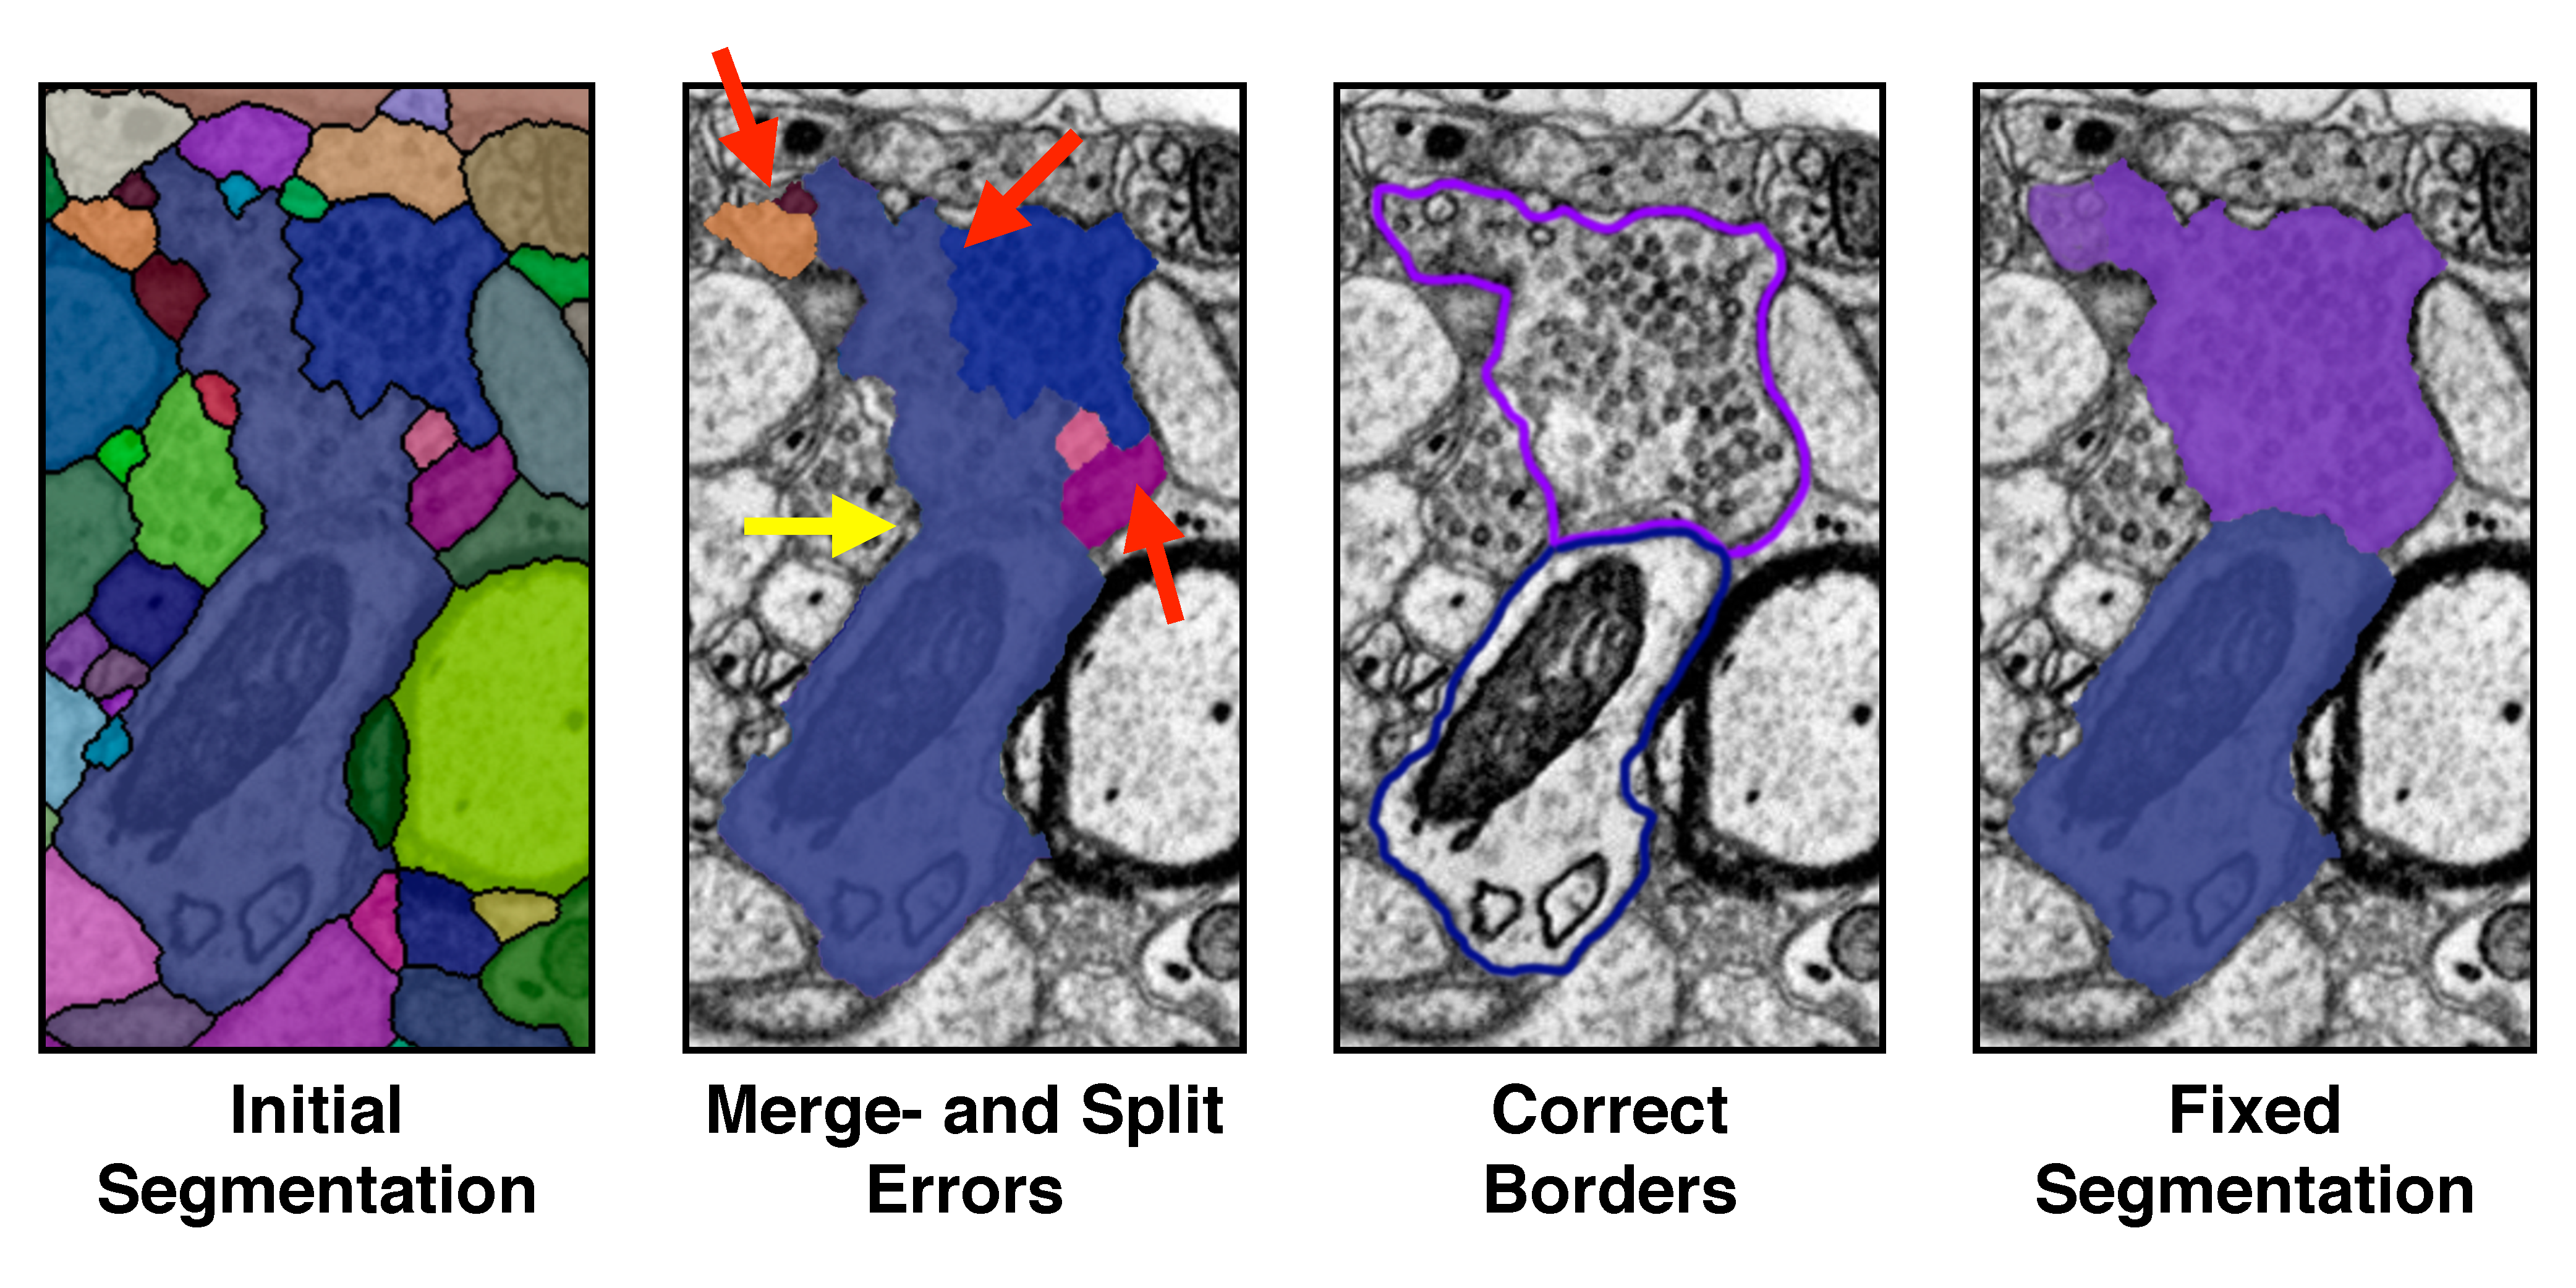
\includegraphics[width=\linewidth]{merge_and_split_errors.pdf}
\end{center}
\vspace{-4mm}
   \caption{The most common proofreading corrections are fixing split errors (red arrows) and merge errors (yellow arrow). A fixed segmentation matches the cell borders.}
\label{fig:merge_and_slit_errors}
\end{figure}

Our goal is to automatically detect potential split and merge errors to reduce visual
inspection time. Further, to reduce correction time, we propose
corrections to the user to accept or reject. We call this process \textit{guided
proofreading}.

We train a classifier for split error detection with a convolutional neural network
(CNN). This takes as input patches of membrane segmentation probabilities, cell
segmentation masks, and boundary masks, and outputs a split-probability score. As we
must process large data, this classifier only operates on cell boundaries, which
reduces computation over methods that analyze every pixel. For merge errors, we
invert and reuse the split classification network, and ask it to rate a
set of generated boundaries that hypothesize a split. 

Possible erroneous regions are sorted by their score, and a candidate correction is generated for each
region. Then, a user works through this list of regions and corrections. In a
forced choice setting, the user either selects a correction or skips it to
advance to the next region. In an automatic setting, errors with a high probability are automatically corrected first, given an appropriate
probability threshold, after which the user would take over. Finally, to test
the limits of performance, we create an oracle which only accepts corrections
that improve the segmentation, based on knowledge of the ground truth. This is
guided proofreading with a perfect user.

We evaluate these methods on multiple connectomics datasets. For the forced
choice setting, we perform a quantitative user study with 20 novice users who
have no previous experience of proofreading EM data. We ask participants to
proofread a small segmentation volume in a fixed time frame. In a
between-subjects design, we compare guided proofreading to the semi-automatic
\textit{focused proofreading} approach by Plaza~\cite{focused_proofreading}. In
addition, we compare against the manual interactive proofreading tool
\textit{Dojo} by Haehn~\etal~\cite{haehn_dojo_2014}. We also asked four domain
experts to use guided proofreading and focused proofreading for comparison.

This paper makes the following contributions.
%
First, we present a CNN-based boundary classifier for split errors, plus a merge
error classifier that inverts the split error classifier. This is used to
propose merge error corrections, removing the need to manually draw the missing
edge. These classifiers perform well without much training data, which is
expensive to collect for connectomics data.
%
Second, we developed a guided proofreading approach to correcting segmentation
volumes, and an assessment scenario comparing forced-choice interaction with
automatic and oracle proofreading.
%
Third, we present the results of a quantitative user study assessing
guided proofreading. Our method is able to reduce segmentation
error faster than state-of-the-art semi-automatic tools for both novice and
expert users.

Guided proofreading is applicable to all existing automatic segmentation methods that
produce a label map. As such, we believe that our approach is a promising
direction to proofread segmentations more efficiently and better tackle large
volumes of connectomics imagery.

\begin{figure*}[t]
\begin{center}
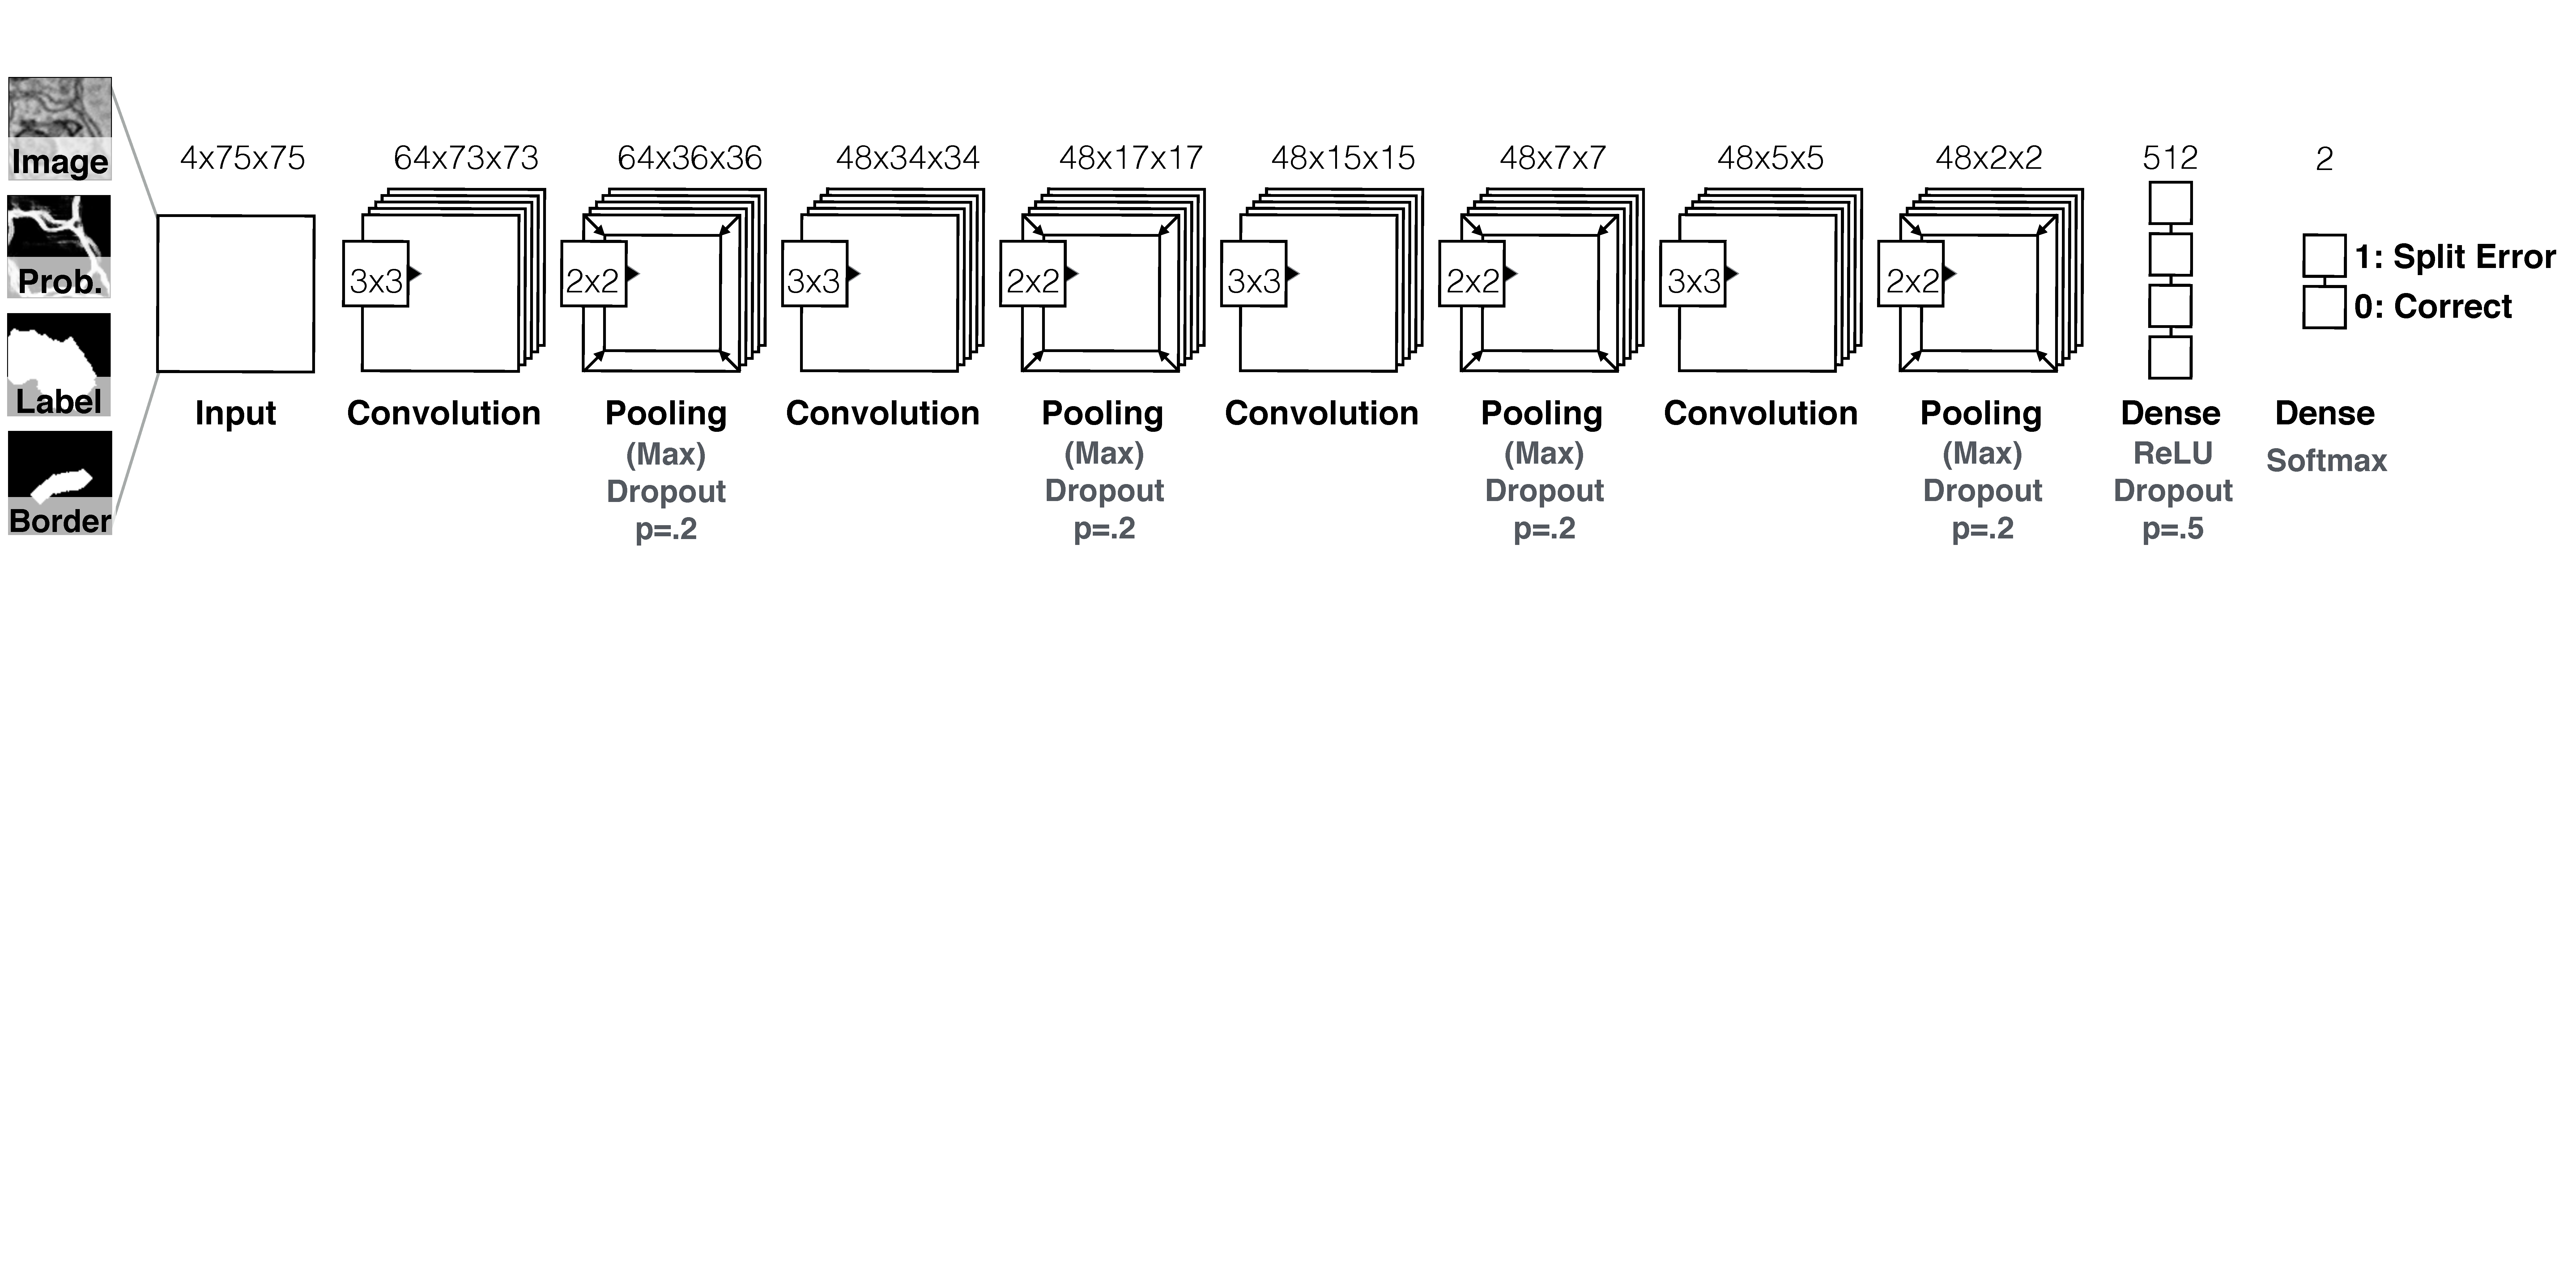
\includegraphics[width=\linewidth]{gfx/architecture.pdf}
\end{center}
  \vspace{-4mm}
   \caption{We build the guided proofreading classifiers using a traditional CNN architecture. The network is based on four convolutional layers, each followed by max pooling as well as dropout regularization. The 4-channel input patches are rated as either correct splits or as split errors.}
\label{fig:architecture}
\end{figure*}

\section{Related Work}

\textbf{Automatic Segmentation.} Multi-terabyte EM brain volumes require automatic segmentation~\cite{jain2010,Liu2014,NunezIglesias2013Machine,GALA2014}, but can be hard to classify due to ambiguous intercellular space: the 2013 IEEE ISBI neurites 3D segmentation challenge~\cite{isbi_challenge} showed that existing algorithms which learn from expert-segmented training data still exhibit high error rates. 

Many works tackle this problem. NeuroProof \cite{neuroproof2013} decreases error rates by learning a agglomeration on over-segmentations of images, based on a random forest classifier. Vazquez-Reina \etal~\cite{amelio_segmentation} take whole EM volumes into account rather than a per section approach, then solve a fusion problem with a global context. Kaynig \etal~\cite{kaynig10} propose a random forest classifier coupled with an anisotropic smoothing prior in a conditional random field framework with 3D segment fusion. Bogovic \etal~\cite{BogovicHJ13} learn 3D features unsupervised, and show that they can be better than by-hand designs. 

It is also possible to learn segmentation classification features directly from images with CNNs. Ronneberger \etal~\cite{RonnebergerFB15} use a contracting/expanding CNN path architecture to enable precise boundary localization with small amounts of training data. Lee \etal~\cite{lee2015recursive} recursively train very deep networks with 2D and 3D filters to detect boundaries.

All these approaches make good progress; however, in general, proofreading is still required to correct errors.
\\~\\
\textbf{Interactive Proofreading.} While proofreading is very time consuming, it is fairly easy for humans to perform corrections through splitting and merging segments. One expert tool is Raveler, introduced by Chklovskii~\etal~\cite{chklovskii2010, raveler}. Raveler is used today by professional proofreaders, and it offers many parameters for tweaking the process. Similar systems exist as products or plugins to visualization systems,~\eg V3D~\cite{proofreading_bottleneck} or AVIZO~\cite{markus_proofreading}. 

Recent papers have attacked the problem of proofreading massive datasets through crowdsourcing with novices~\cite{saalfeld09,anderson2011,Giuly2013DP2}. One popular platform is EyeWire, by Kim \etal~\cite{eyewire_nature}, where participants earn virtual rewards for merging oversegmented labeling to reconstruct retina cells.

Between expert systems and online games sit Mojo and \textit{Dojo}, by Haehn \etal~\cite{haehn_dojo_2014,Neuroblocks}, which use simple scribble interfaces for error correction. Dojo extends this to distributed proofreading via a minimalistic web-based user interface. The authors define requirements for general proofreading tools, and then evaluate the accuracy and speed of Raveler, Mojo, and Dojo through a quantitative user study (Sec. 3 and 4)~\cite{haehn_dojo_2014}. Dojo had the highest performance. In this paper, we use Dojo as a baseline for interactive proofreading, and so we extend the Haehn \etal experiment.

All interactive proofreading solutions require the user to find potential errors manually, which takes the majority of the time~\cite{proofreading_bottleneck,haehn_dojo_2014}. Recent works propose computer-aided proofreading systems which help reduce the time spent in this visual search task.
\\~\\
\textbf{Computer-aided Proofreading.} Uzunbas \etal showed that potential labeling errors can be found by considering the merge tree of an automatic segmentation method~\cite{uzunbas}. The authors track uncertainty throughout the automatic labeling by training a conditional random field. This segmentation technique produces uncertainty estimates, which can be used to present potential regions for proofreading to the user. While it works on isotropic volumes, more work is needed to apply it to anisotropic volumes, like most connectomics datasets.

%Their method requires further work to overcome the requirement of isotropic volumes, a property not given for most connectomics datasets. Our approach, guided proofreading, works on isotropic as well as anisotropic data, and finds merge and split errors.

Karimov \etal propose guided volume editing~\cite{karimov_guided_volume_editing}, which measures the difference in histogram distributions in image data to find potential split and merge errors in the corresponding segmentation. This lets expert users correct labeled computer-tomography datasets, using several interactions per correction. To correct merge errors, the authors create a large number of superpixels within a single segment and then successively group them based on dissimilarities. We were inspired by this approach but generate single watershed boundaries to handle the intracellular variance in high-resolution EM images (Sec. \ref{sec:methods}).

Most closely related to our approach is the work of Plaza, who proposed \textit{focused proofreading}~\cite{focused_proofreading}. This method generates affinity scores by analyzing a region adjacency graph across slices, then finds the largest affinities based on a defined impact score. This yields edges of potential split errors which can be presented to the proofreader. Plaza reports that additional manual work is required to find and correct merge errors. Focused proofreading builds upon NeuroProof \cite{neuroproof2013} as its agglomerator, and is open source with integration into Raveler. As the closest related work, we wish to use this method as a baseline to evaluate our approach (Sec.~\ref{sec:evaluation}). However, as Haehn \etal showed that Raveler is less performant than Dojo for novice users, we separate the backend affinity score calculation from the expert-level front end, and present our own interface (Sec.~\ref{sec:evaluation}).





\section{Method}
\label{sec:methods}

%We first describe our classifier for detecting split errors which is based on a convolutional neural network (CNN). We detail the CNN architecture, input features and the training method. We then describe how the same classifier can be used to detect merge errors and how we create potential corrections. The classifiers are integrated into an existing proofreading workflow as reported after. Finally, we explore an active label suggestion method which reorders the ranking obtained by our classifiers and maximizes the information gain provided by each potential correction.
\subsection{Split Error Detection}

We build a split error classifier with output $p$ using a CNN to check whether an edge within an existing automatic segmentation is valid ($p=0$) or not ($p=1$). Rather than analyzing every input pixel, the classifier operates only on segment boundaries, which requires less pixel context and is faster. In contrast to Bogovic \etal~\cite{BogovicHJ13}, we work with 2D slices rather than 3D volumes. This enables proofreading prior or in parallel to a computationally expensive stitching and 3D alignment of individual EM images.
\\~\\
\textbf{Convolutional Neural Network Architecture.} Split error detection of a given boundary is a binary classification task since the boundary is either correct or erroneous. However, in reality, the score $p$ is between 0 and 1. The classification complexity arises from hundreds of different cell types in connectomics data rather than from the classification decision itself. Intuitively, this yields a wider architecture with more filters rather than a deeper architecture with more layers. We explored different architectural configurations---including residual networks~\cite{resnet}---by performing a brute force parameter search and comparing precision and recall (see supplementary materials). Our final CNN configuration for split error detection is composed of four convolutional layers, each followed by max pooling as well as dropout regularization to prevent overfitting due to limited training data (Fig.~\ref{fig:architecture}).
\\~\\
\textbf{Classifier Inputs.} To train the CNN, we consider boundary context in the decision making process by using a $75\times75$ pixel patch at the center of an existing boundary. This size covers approximately $80\%$ of all boundaries in the 6~nm Mouse S1 AC3 Open Connectome Project dataset. If the boundary length is not fully covered, we sample up to 10 non-overlapping patches along the boundary, and combine the resulting score by averaging weighted by the boundary length coverage per patch.

Similar to Bogovich~\etal~\cite{BogovicHJ13}, we use grayscale image data,
corresponding boundary probabilities, and a single binary mask combining the two
neighboring labels as inputs to our CNN. However, we observed that the
boundary probability information generated from EM images is often misleading
due to noise or artifacts in the data. This can result in merge errors within
the automatic segmentation. To better direct our classifier to train on the true
boundary, we extract the border between two segments. Then, we dilate this border
by 5 pixels to consider slight edge ambiguities and use this binary mask as an
additional input. This creates a stacked 4-channel input patch.
Fig.~\ref{fig:cnn_inputs} shows examples of correct and erroneous input
patches and their corresponding automatic segmentation and ground truth.

\begin{figure}[t]
\begin{center}
  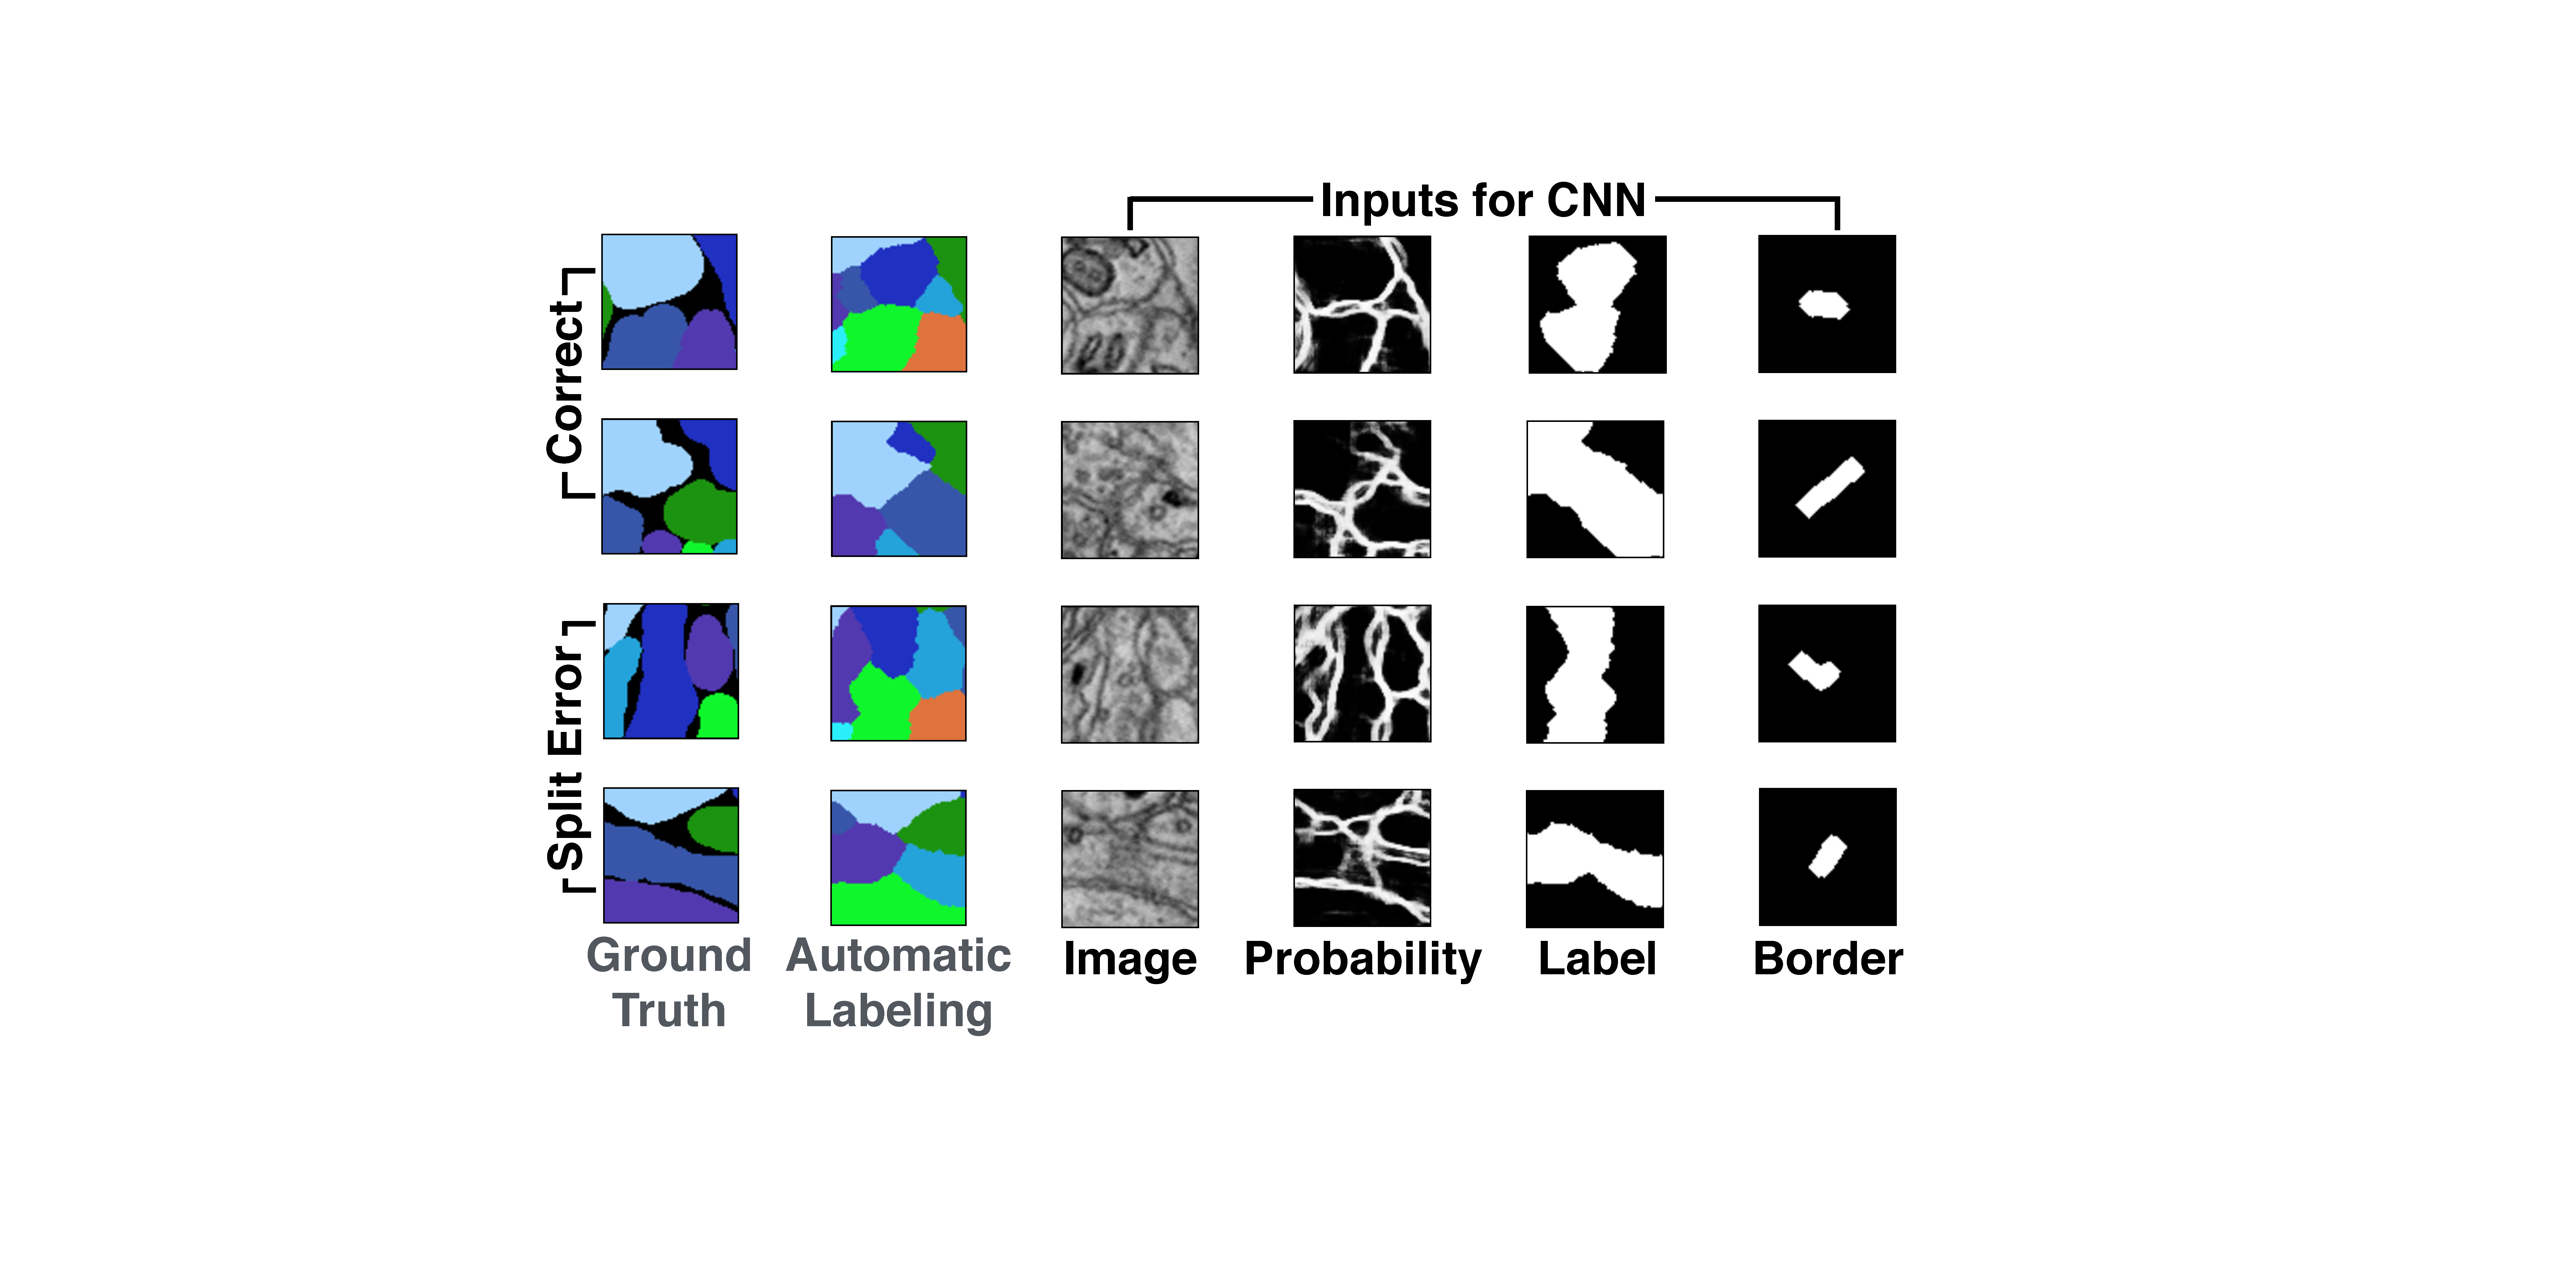
\includegraphics[width=\linewidth]{gfx/cnn_inputs.pdf}
\end{center}
 % \vspace{-4mm}
   \caption{Example inputs for learning correct splits and split errors, as per a candidate segmentation versus the ground truth. Image, membrane probabilities, merged binary labels, and a dilated border mask provide 4-channel input patches.}
\label{fig:cnn_inputs}
\end{figure}


\subsection{Merge Error Detection}

Identification and correction of merge errors is more challenging than finding and fixing split errors, because we must look inside segmentation regions for missing or incomplete boundaries and then propose the correct boundary. However, we can reuse the same trained CNN for this task. Similar to guided volume editing by Karimov~\etal~\cite{karimov_guided_volume_editing}, we generate potential borders within a segment. For each segmentation label, we dilate the label by 20 pixel and generate 50 potential boundaries through the region by randomly placing watershed seed points at opposite sides of the label boundary. We perform watershed on the inverted grayscale EM image. This yields 50 candidate splits.

Dilation of the segment prior to watershed is motivated by our observation that the generated splits tend to attach to real membrane boundaries. These boundaries are then individually rated using our split error classifier. For this, we invert the probability score such that a correct split (previously encoded as $p=0$) is most likely a candidate for a merge error (now encoded as $p=1$). In other words, if a generated boundary is ranked as correct, it probably should be in the segmentation. Fig. \ref{fig:merge_error} illustrates this procedure.

\begin{figure}[t]
\begin{center}
  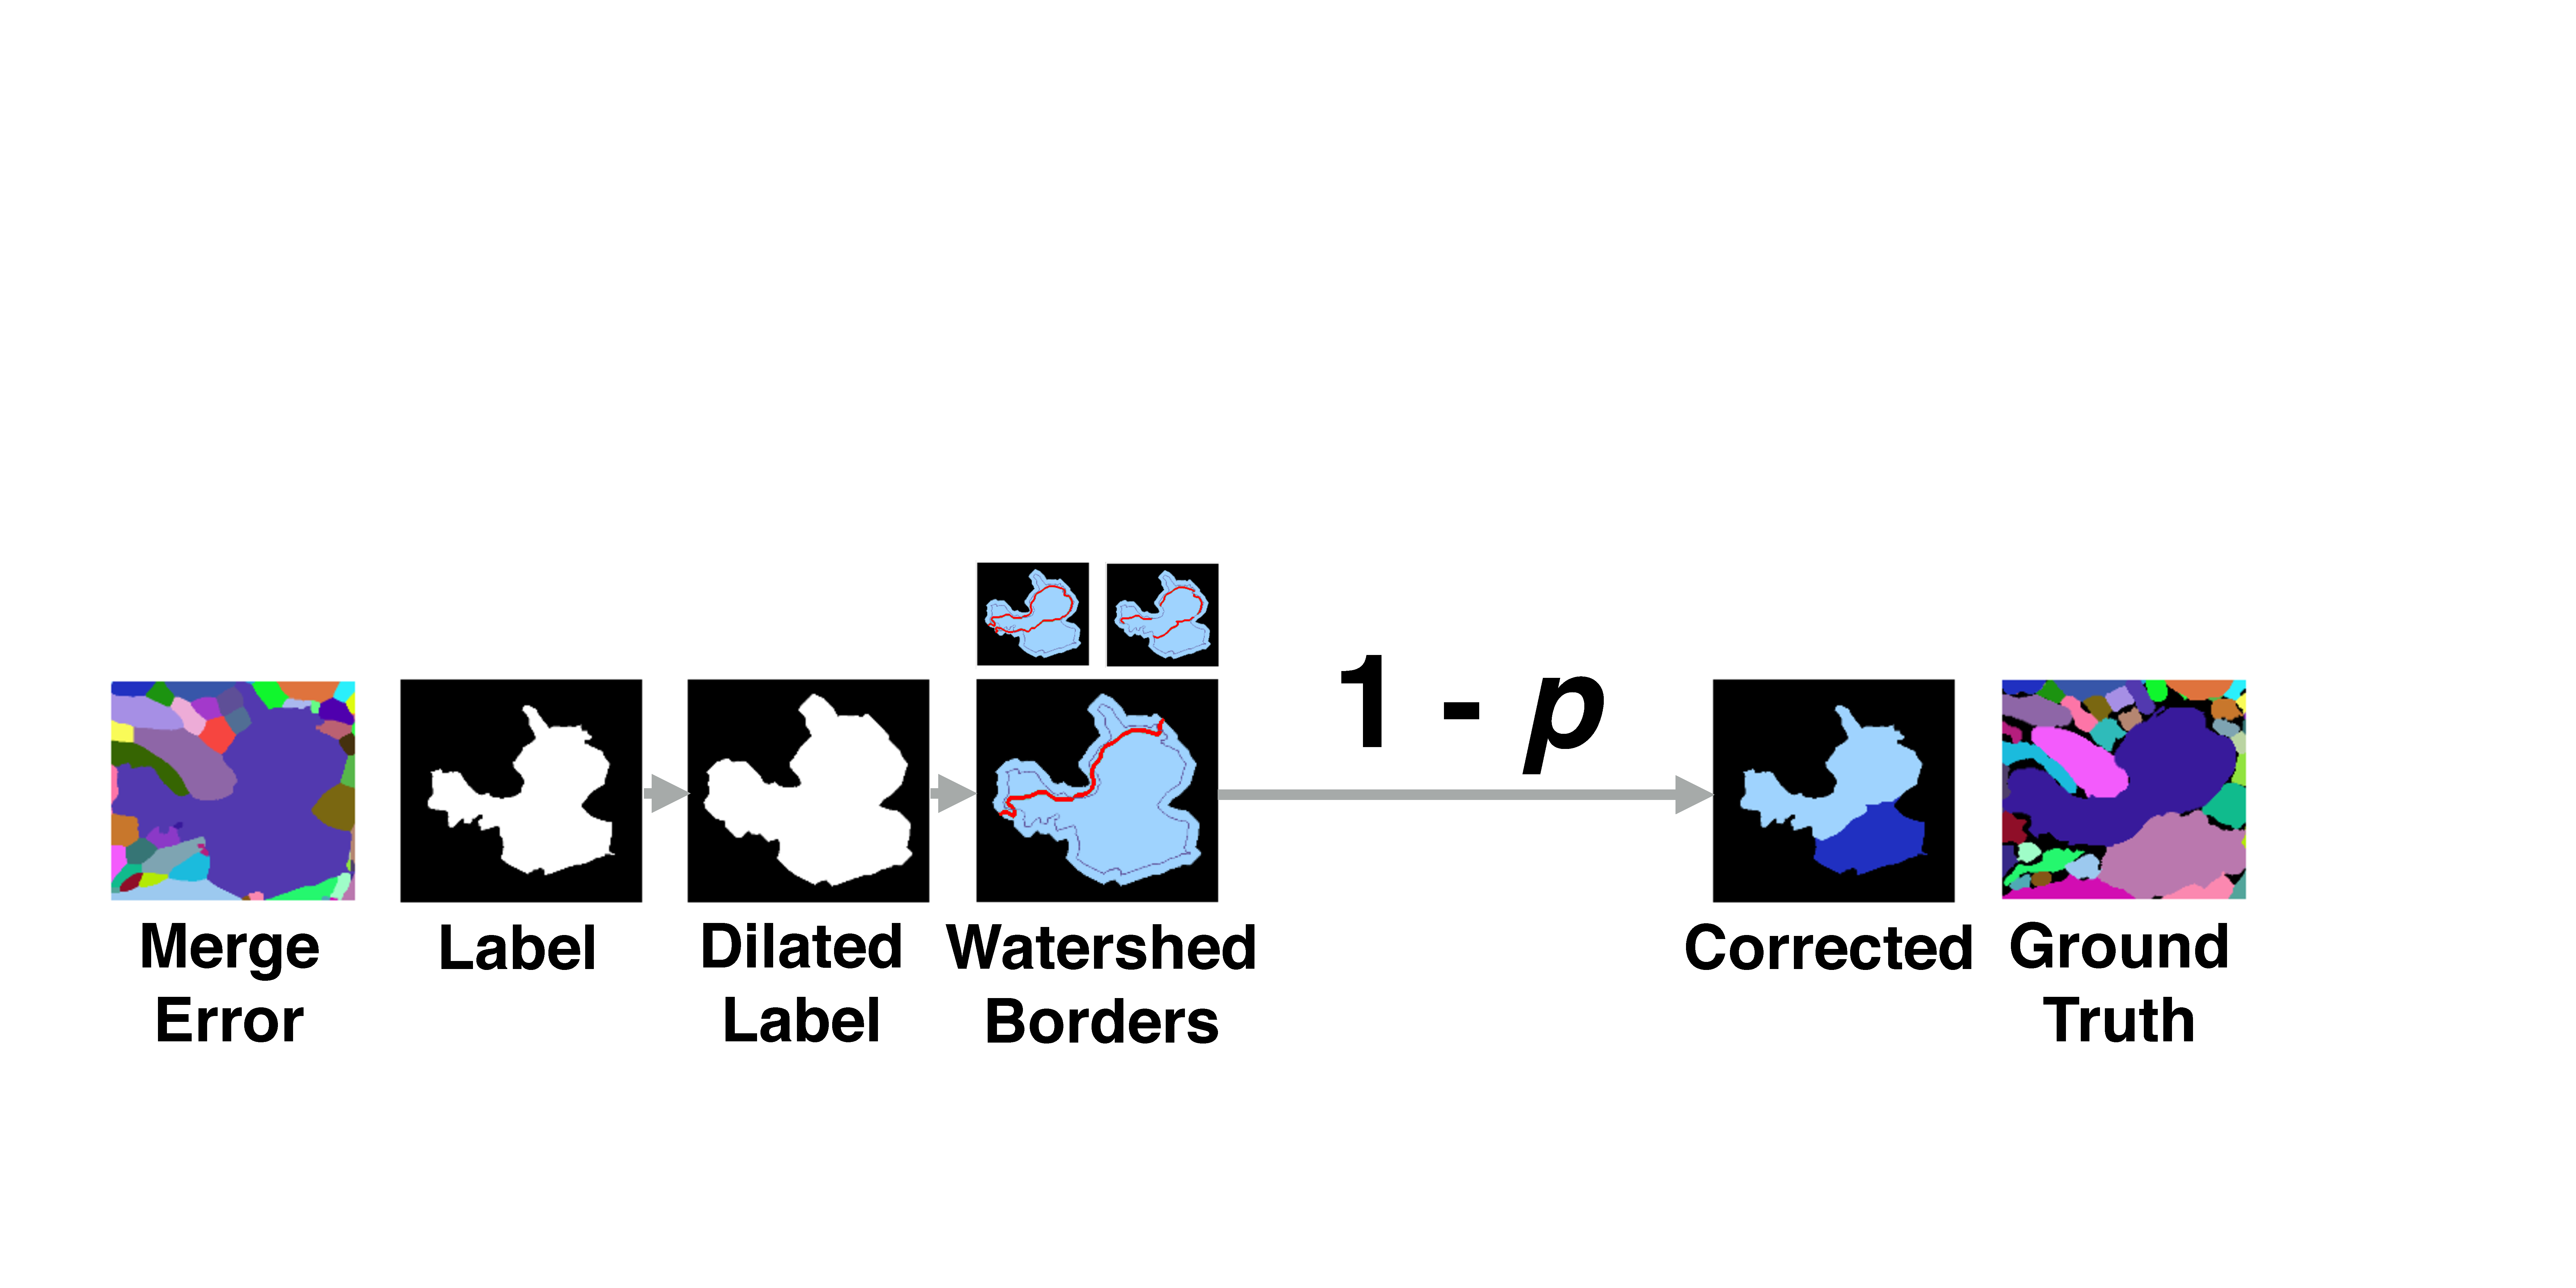
\includegraphics[width=\linewidth]{gfx/merge_error.pdf}
\end{center}
%  \vspace{-4mm}
   \caption{Merge errors are identified by generating randomly-seeded watershed borders within a dilated label segment. Then, each border is individually rated using the split error CNN by inverting the probability score. A confident rating for a correct split most likely indicates the missing border of the merge error, and can be used to correct the labeling.\JT{Candidate to improve.}}
\label{fig:merge_error}
\end{figure}

\subsection{Error Correction}
\label{sec:errorcorrection}

We use the proposed classifiers in combination to perform corrections of split and merge errors in automatic segmentations. For this, we first perform merge error detection for all existing segments in a dataset and store the inverted rankings $1-p$ as well as potential corrections. After that, we perform split error detection and store the ranking $p$ for all neighboring segments in the segmentation. Then, we sort the merge and split error rankings separately from highest to lowest. For error correction, first we loop through the potential merge error regions and then through the potential split error regions. During this process, each error is now subject to a yes/no decision which can be provided in different ways:

\paragraph{Selection oracle.} If ground truth data is available, the selection oracle \textit{knows} whether a possible correction improves an automatic segmentation. This is realized by simply comparing the outcome of a correction using a defined measure. The oracle only accepts corrections which improve the automatic segmentation---others get
discarded. This is guided proofreading with a perfect user, and allows us to assess the upper limit of performance.

\paragraph{Automatic selection with threshold.} The decision whether to accept or reject a potential correction is taken by comparing rankings to a threshold $p_t$. If the inverted score $1-p$ of a merge error is higher than a threshold $1-p_t$, the correction is accepted. Similarly, a correction is accepted for a split error if the ranking $p$ is higher than $p_t$. Our experiments have shown that the threshold $p_t$ is the same for merge and split errors for a balanced classifier that has been trained on equal numbers of correct and error patches.

\paragraph{Forced choice setting.} We present a user with the choice to accept or reject a correction. All potential split errors are seen. Inspecting all merge errors is not possible for users due to the sheer amount of generated borders. Therefore, we only present merge errors that satisfy $1-p_t$.

\noindent \newline In all cases, a decision has to be made to advance to the next possible erroneous region. If a merge error correction was accepted, the newly found boundary is added to the segmentation data. This partially updates the merge error and split error ranking with respect to the new segment. If a split error correction was accepted, two segments are merged in the segmentation data and the disappearing segment is removed from all error rankings. Then, we perform merge error detection on the now larger segment and update the ranking. We also update the split error rankings to include all new neighbors, and re-sort. The error with the next highest ranking then forces a choice.

\subsection{User Interface}

Our guided proofreading is integrated into an existing workflow for large connectomics data. The system is web-based and is designed with a novice-friendly user interface (Fig.~\ref{fig:ui}). We show the outline of the current labeling of a cell boundary and its proposed correction overlaying the EM image data. For the user, it is not possible to distinguish the current labeling and the proposed correction to avoid selection bias. We also show a solid overlay of the current and the proposed labeling. In addition, we show the image without overlays to provide an unoccluded view. User interaction is simple and involves one mouse click on either the current labeling or the correction. After interaction, the next potential error is shown.

\begin{figure}[t]
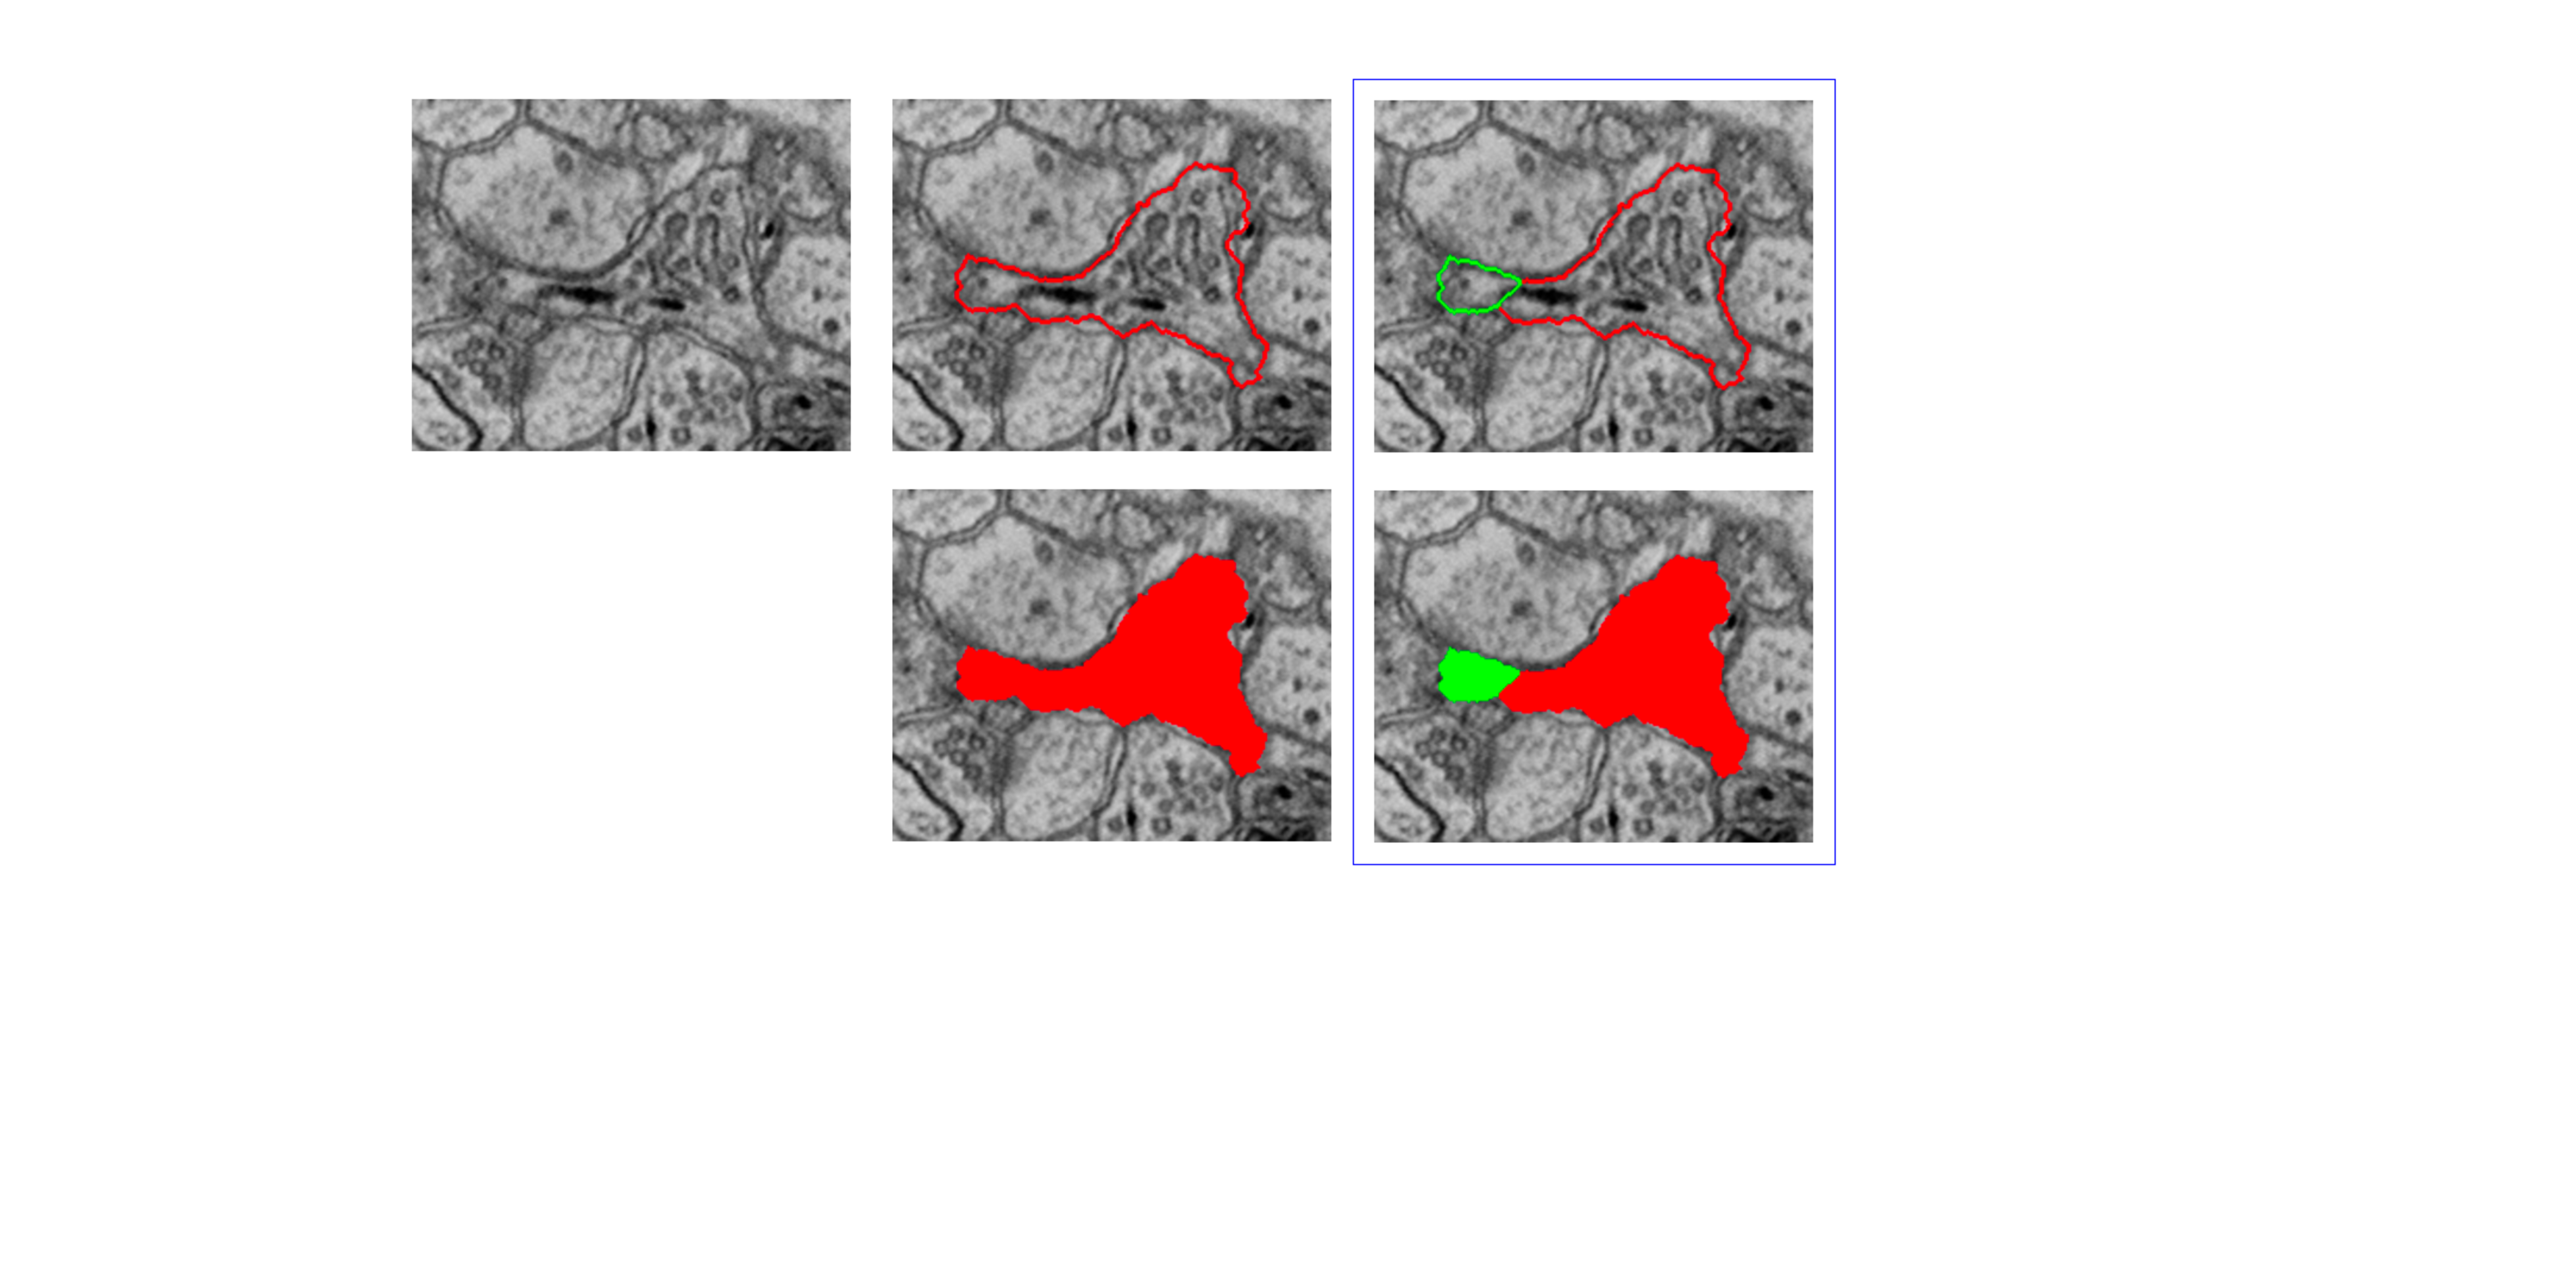
\includegraphics[width=\linewidth]{gfx/user_interface_split.pdf}
\caption{Our guided proofreading user interface. A candidate error region is shown on the left. The user must choose between the region being a split error which needs correcting (center) or not (right). Hovering highlights the current selection with a yellow border, and a mouse click confirms the choice and advances to the next potential error.\JT{Needs labels on the images; also, removal of black background.}}
\label{fig:ui}
\end{figure}

%
%\subsection{Active Label Suggestion}
%
%In an interactive setting, one way to present patches to the user for proofreading is to order them by the confidence probability of the GP classifier. However, in an active learning setting, where the network is retrained repeatedly on new label evidence, this approach is less likely to decrease segmentation error as, with the new labels, we are only reinforcing what the network already has a high confidence in.
%Instead, we apply active label suggestion to guide the user into labeling patches which will be more informative to retraining, and so overall decrease VI faster within the proofreading cycle of label $\rightarrow$ train $\rightarrow$ label. For each patch, we remove the softmax classification layer and look at the activation weights associated with the last dense layer. These become a high-dimensional feature vector. Then, we adapt Anon~\etal~\cite{ANON} to provide label suggestions based on features from the learned CNN, which is based on maximizing the average information gain provided by a candidate patch to label.
%A second consideration is that each patch labeled by the user provides evidence to other patches, e.g., correcting a split error redefines an entire boundary, from which multiple candidate patch labelings could have been drawn. As such, when the user labels a patch, we consider all `knock-on' effect patches as also being labeled, and feed these into the active label suggestion system similarly.
%In section \ref{sec:evaluation}, we report the difference in performance from using active label suggestion rather than confidence ordering when presenting patches to the user. These results are without retraining the network after new labelings: this should improve results, but would have to be batched to reduce computational load; hence, we leave this for future work.


%\begin{figure*}[t]
%\begin{center}
%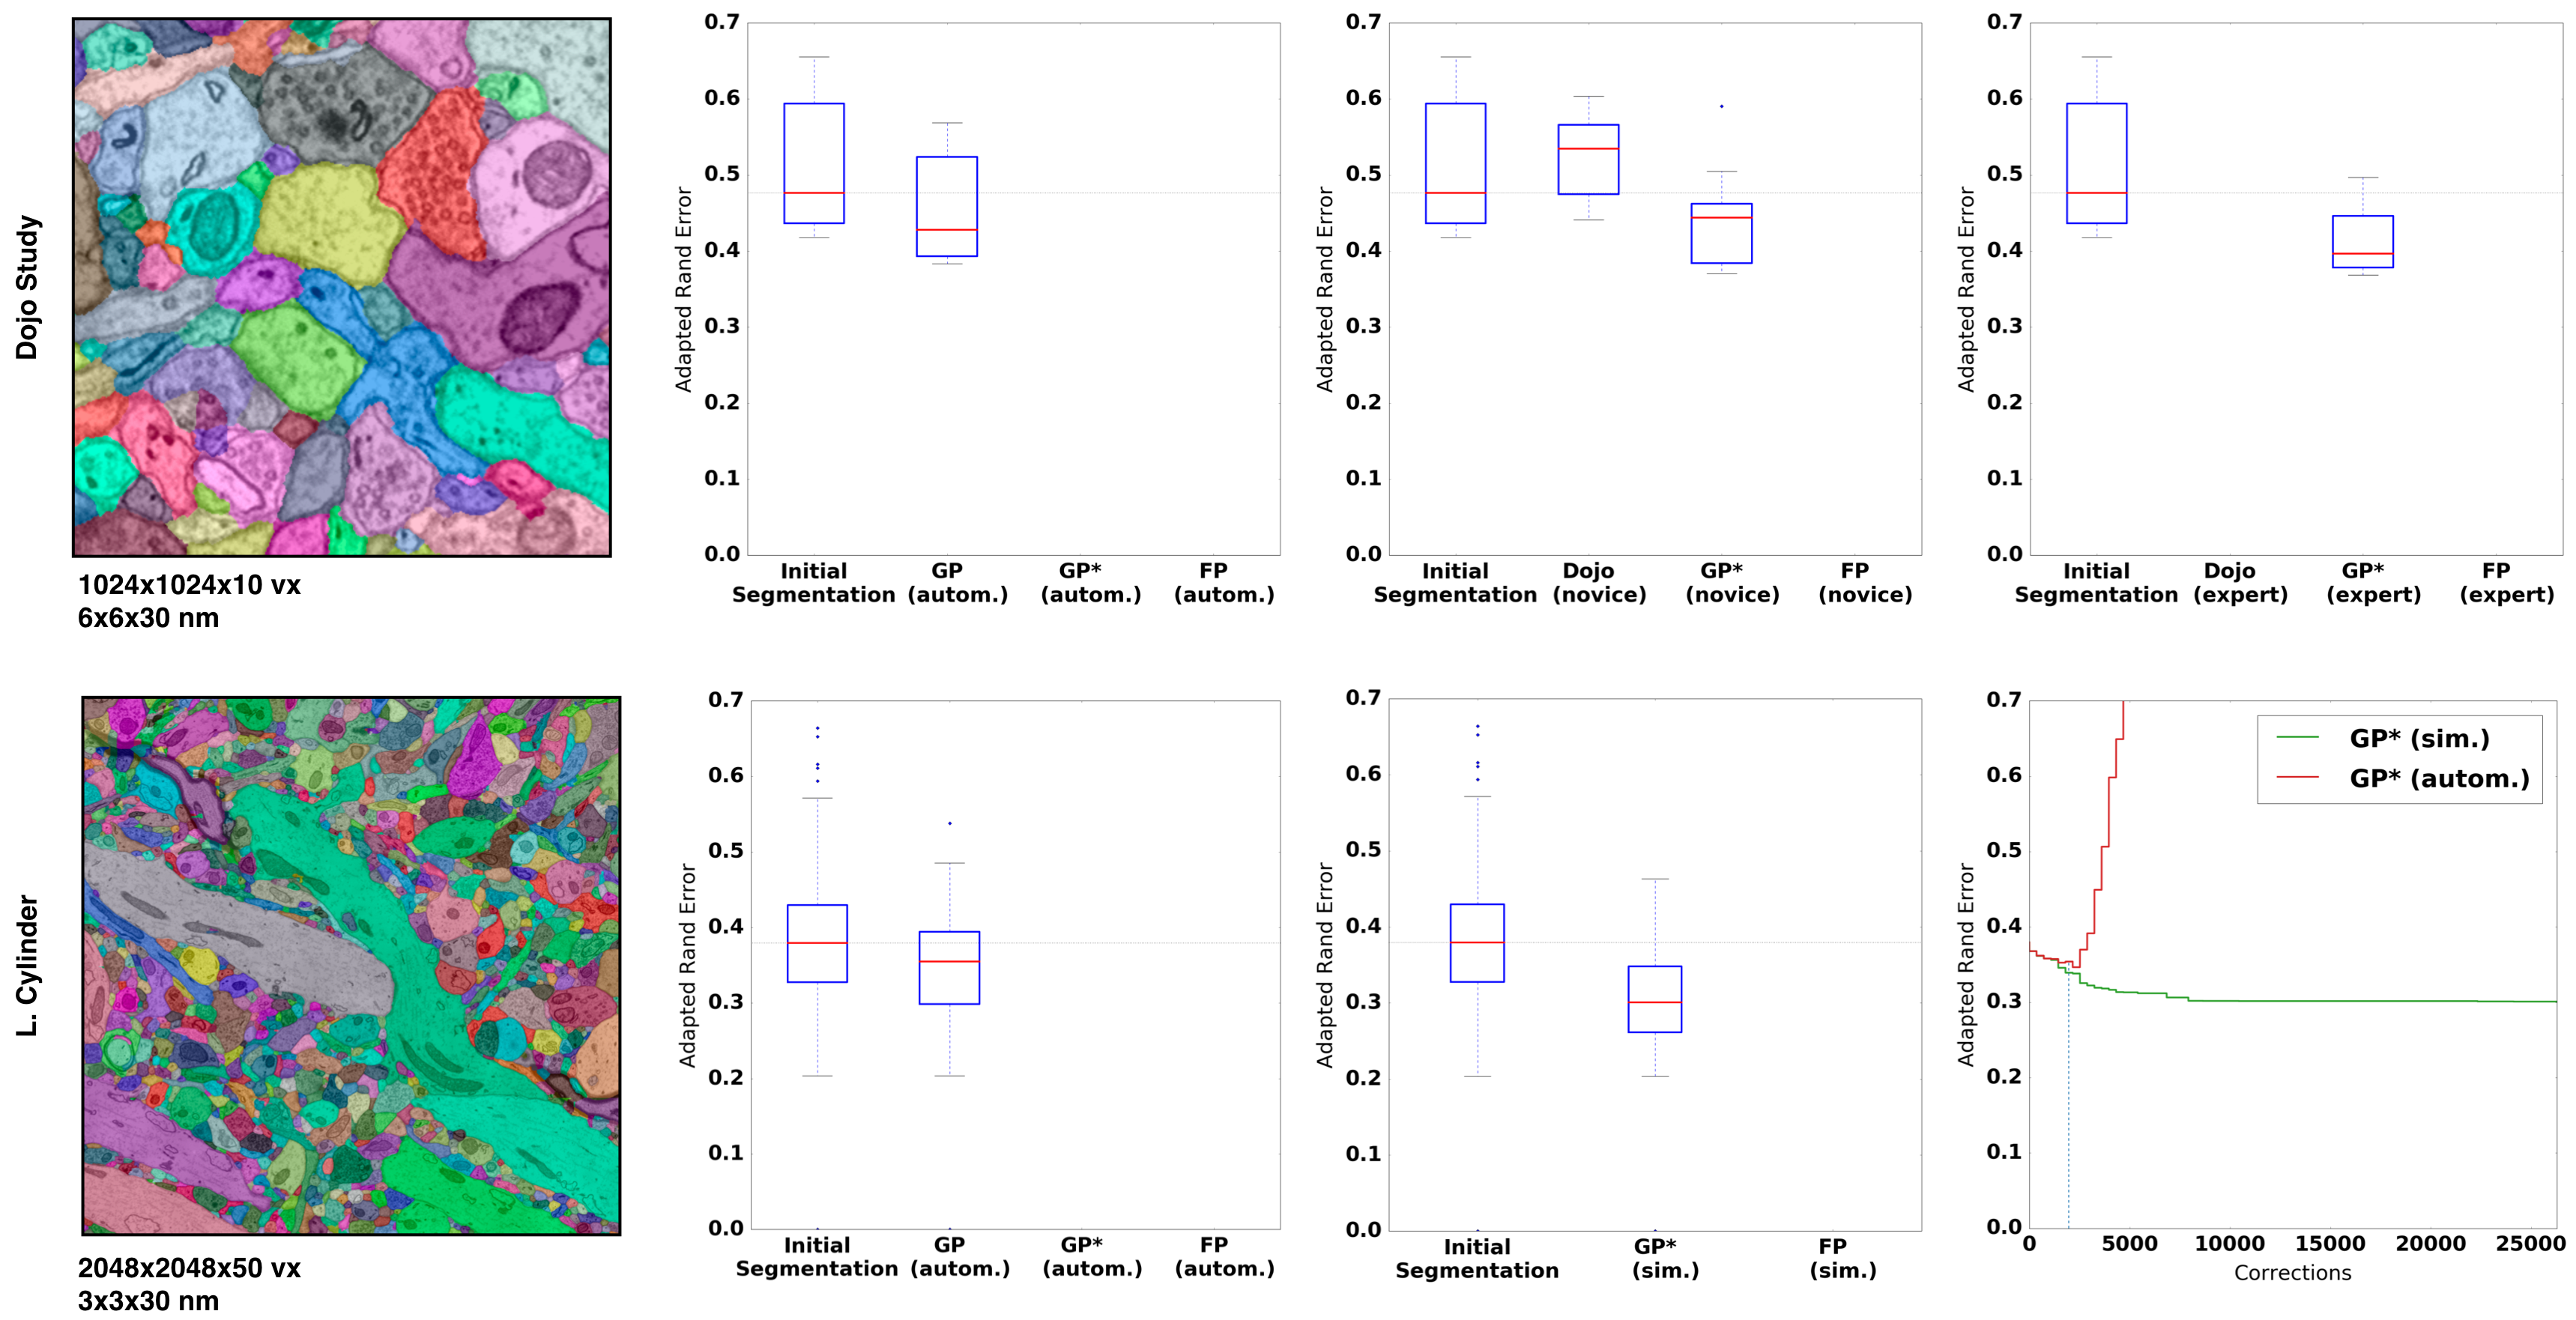
\includegraphics[width=\linewidth]{gfx/results_mouse.png}
%\end{center}
%  \vspace{-4mm}
%   \caption{Performance evaluation of the classifiers on two mouse brain datasets measured as adapted Rand error (lower scores are better). We compare guided proofreading (GP), guided proofreading with active label suggestion (GP*) and focused proofreading. Proofreading is performed automatically (autom., with probability threshold $p_t=.95$), simulated as a perfect user (sim.), or by novice and expert users as indicated. The first row of images shows the results of a user study and includes comparisons to the interactive proofreading software Dojo by Haehn \etal \cite{haehn_dojo_2014}. GP* is able to correct the segmentation further than other methods. The second row shows the results of the simulated user compared to automatic GP* and FP performance. The bottom right graph compares automatic GP* and simulated GP* per individual correction. The blue dashed line here indicates the moment the probability threshold $p_t$ is reached. The simulated user is able to correct the initial segmentation beyond this threshold while automatic GP* then introduces errors.}
%\label{fig:results_mouse}
%\end{figure*}

\section{Evaluation}
\label{sec:evaluation}

We evaluate guided proofreading on multiple different real-world connectomics datasets of different species. All datasets were acquired using either serial section electron microscopy (ssEM) or serial section transmission electron microscopy (ssTEM). We perform experiments with the selection oracle, with automatic selection with threshold, and in the forced choice setting via a between-subjects user study with both novice and expert participants.

\subsection{Datasets}

\paragraph{L. Cylinder.} We use the left part of the 3-cylinder mouse cortex volume of Kasthuri \etal~\cite{kasthuri2015saturated} ($2048\times2048\times300$ voxels). The tissue is dense mammalian neuropil from layers 4 and 5 of the S1 primary somatosensory cortex, acquired using ssEM. The dataset resolution is $3\times3\times30~\text{nm}^3\text{/voxel}$. Image data and a manually-labeled expert `ground truth' segmentation is publicly available\footnote{\scriptsize{\url{https://software.rc.fas.harvard.edu/lichtman/vast/}}}.

\paragraph{AC4 subvolume.} This is part of a publicly-available dataset of mouse cortex that was published for the ISBI 2013 challenge ``SNEMI3D: 3D Segmentation of neurites in EM images''. The dataset resolution is $6\times6\times30~\text{nm}^3\text{/voxel}$ and it was acquired using ssEM. Haehn~\etal~\cite{haehn_dojo_2014} found the most representative subvolume ($400\times400\times10$ voxels) of this dataset with respect to the distribution of object sizes, and used it for their interactive connectomics proofreading tool experiments. We use their publicly available data, labeled ground truth, and study findings\footnote{\scriptsize{\url{http://rhoana.org/dojo/}}}.

%\paragraph{CREMI A/B/C.} As part of the MICCAI 2016 challenge on circuit reconstruction from electron microscopy images (CREMI), six ssTEM datasets were made publicly available\footnote{\scriptsize{\url{http://www.cremi.org}}},  each $1250\times1250\times125$ voxels. Since only three datasets include manually-labeled `ground truth', we use these three volumes for our experiments. The volumes are part of an adult fruit fly (Drosophila melanogaster) brain. The resolution of all three datasets is $4\times4\times40~\text{nm}^3\text{/voxel}$.

\paragraph{Automatic segmentation pipeline.}
We use a state-of-the-art method to create a dense automatic segmentation of the data. Membrane probabilities are generated using a CNN based on the U-net architecture (trained exclusively on different data than the GP classifiers)~\cite{RonnebergerFB15}. The probabilities are used to seed watershed and generate an oversegmentation using superpixels. Agglomeration is then performed by the GALA active learning classifier with a fixed agglomeration threshold of 0.3~\cite{nunez2014graph}. We describe this approach in the supplemental material.

\subsection{Classifier Training}

We train our split error classifier on the L. Cylinder dataset. We use the first 250 sections of the data for training and validation. For n-fold cross validation, we select one quarter of this data and re-select after each epoch. We minimize cross-entropy loss and update using stochastic gradient descent with Nesterov momentum~\cite{nesterov}. To generate training data, we identify correct regions and split errors in the automatic segmentation by intersection with ground truth regions. This is required since extracellular space is not labeled in the ground truth, but is in our dense automatic segmentation. From these regions, we sample 112,760 correct and 112,760 split error patches with 4-channels (Sec.~\ref{sec:spliterrordetection}). The patches are normalized. To augment our training data, we rotate patches within each mini-batch by $k*90$ degrees with randomly chosen integer $k$. The training parameters such as filter size, number of filters, learning rate, and momentum are the result of intuition and experience, studying recent machine learning research, and a limited brute force parameter search (see supplementary material). 

Table~\ref{tab:parameters} lists the final parameters. Our CNN configuration results in 171,474 learnable parameters. We assume that training has converged if the validation loss does not decrease for 50 epochs. We test the CNN by generating a balanced set of 8,780 correct and 8,780 error patches using unseen data of the left cylinder dataset. 

\begin{table}[t]
\caption{Training parameters, cost, and results of our guided proofreading classifier versus focused proofreading by Plaza~\cite{focused_proofreading}. Both methods were trained on the same mouse brain dataset using the same hardware (Tesla X GPU).}%While the training of our classifier is more expensive, testing accuracy is superior. }

\small{
\begin{tabular}{ll}
	\toprule
	\begin{tabular}{l}
		\textbf{Guided Proofreading} \\ \midrule
		\emph{Parameters} \\ \midrule
		Filter size: 3x3 \\ No. Filters 1: 64 \\ No. Filters 2--4: 48 \\ Dense units: 512 \\ Learning rate: 0.03--0.00001\\ Momentum: 0.9--0.999\\Mini-Batchsize: 128 \\
	\end{tabular}
	&
	\begin{tabular}{l}
		\vspace{0.2mm} \\
		\midrule
		\emph{Results---Test Set} \\ \midrule Cost [m]: 383 \\ Val. loss: 0.0845 \\ Val. acc.: 0.969 \\ Test. acc.: 0.94 \\ Prec./Recall: 0.94/0.94 \\ F1 Score: 0.94 \\ ~ \\
	\end{tabular}
\end{tabular}

\vspace{0.5mm}
\begin{tabular}{ll}
	\toprule
	\begin{tabular}{l}
		\textbf{Focused Proofreading}\\ \midrule
		\emph{Parameters} \\ \midrule
		Iterations: 3 \\
		Learning strategy: 2\\
		Mito agglomeration: Off~~~~~~ \\  % Crappy alignment spacing
		Threshold: 0.0\\~\\
	\end{tabular}
	&
	\begin{tabular}{l}
		\vspace{0.2mm} \\
		\midrule
		\emph{Results---Test Set} \\ \midrule Cost [m]: 217 \\ Val. acc.: 0.99 \\ Test. acc.: 0.68 \\ Prec./Recall: 0.58/0.56 \\ F1 Score: 0.54 \\
	\end{tabular}
%	\bottomrule
\end{tabular}
\hrule
}
\label{tab:parameters}
\end{table}

\subsection{Baseline Comparisons}

\paragraph{Interactive proofreading.} Haehn~\etal's comparison of interactive proofreading tools concludes that novices perform best when using Dojo~\cite{haehn_dojo_2014}. We studied the publicly available findings of their user study and use the data of all Dojo users in aggregate as a baseline.

\paragraph{Computer-aided proofreading.} We compare against focused proofreading by Plaza~\cite{focused_proofreading}. Focused proofreading performs graph analysis on the output from NeuroProof~\cite{neuroproof2013}, instead of our GALA approach. Therefore, for training our focused proofreading baseline, we replace GALA in our automatic segmentation pipeline with NeuroProof but use exactly the same input data including membrane probabilities. We obtained the best possible parameters for NeuroProof by consulting the developers (Tab.~\ref{tab:parameters}). Rather than using Raveler as the frontend, we use our own interface (Fig.~\ref{fig:ui}) to compare only the classifier from Plaza's approach.

\subsection{Experiments}

\paragraph{Selection oracle evaluation.} We use the selection oracle as described in Sec.~\ref{sec:errorcorrection} for the decision whether to accept or reject a correction. The purpose of this experiment is to investigate how many corrections are required to reach the best possible outcome. This is a direct comparison of the guided proofreading and focused proofreading classifiers but can only be performed if ground truth data is available. We perform this experiment on all datasets listed above.

\paragraph{Automatic method evaluation.} For this experiment, we accept all suggested corrections if the rankings are above a configured threshold $p_t=.95$ (Sec.~\ref{sec:errorcorrection}). We observed this value as stable in previous experiments with the guided proofreading classifiers (see supplementary material). We compare against the focused proofreading classifier and perform this experiment on all reported datasets.

\paragraph{Forced choice user experiments.} We conducted a quantitative user study to evaluate the forced choice setting (Sec.~\ref{sec:errorcorrection}). In particular, we evaluated how participants perform while correcting an automatic segmentation using the guided proofreading and focused proofreading tools. We designed a single factor between-subjects experiment with the factor \textit{proofreading classifier}, and asked participants to proofread the AC4 subvolume in a fixed time frame of 30 minutes.
To enable comparison against the interactive proofreading study by~Haehn~\etal~\cite{haehn_dojo_2014}, we use the exact same study conditions, dataset, and time limit. The experiment was performed on a machine with standard off-the-shelf hardware. All participants received monetary compensation.

\paragraph{Novice study design.} We recruited participants with no experience in electron microscopy data or proofreading through flyers, mailing lists, and personal interaction. Based on sample size calculation theory, we estimated the study needed ten users per proofreading tool including four potential dropouts~\cite{samplesize1,samplesize2}. All twenty participants completed the study ($N=20$, 10 female; 19-65 years old, $M$=30). 

Each study session began with a five minute standardized explanation of the task. Then, the participants were asked to perform a 3 minute proofreading task on separate but representative data using focused proofreading. The participants were allowed to ask questions during this time. The classifier did not matter in this case since the user interface was the same. The experimenter then loaded the AC4 subvolume with initial pre-computed classifications by either guided proofreading or focused proofreading depending on assignment. After 30 minutes, the participants completed the raw NASA-TLX standard questions for task evaluation~\cite{NASATLX}.
\begin{figure*}[t]
\centering
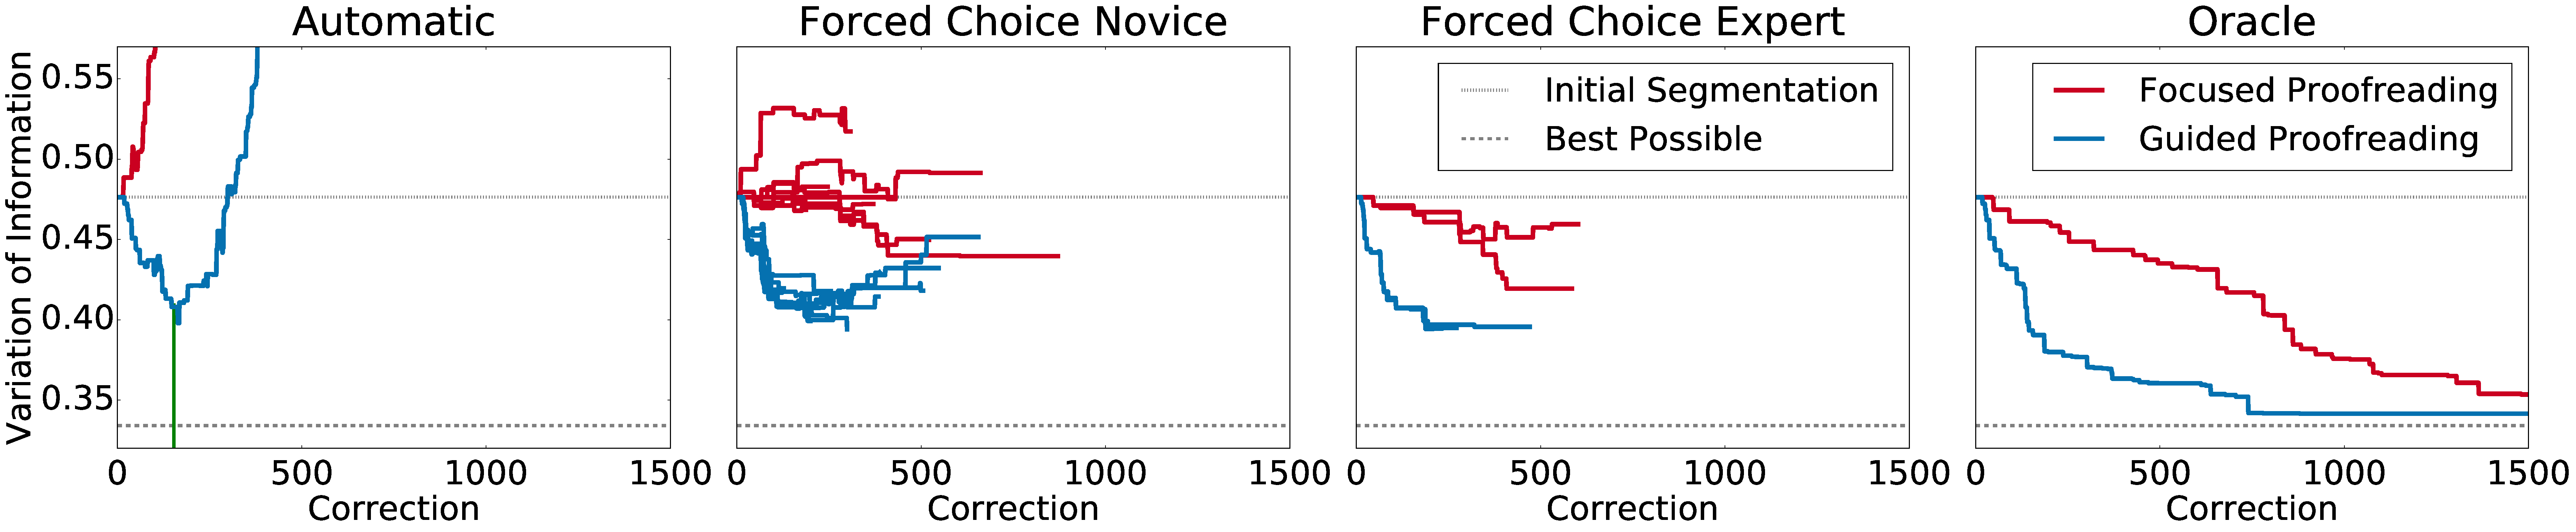
\includegraphics[width=\linewidth]{gfx/ac4trails_combined.pdf}
\caption{Performance comparison of Plaza's focused proofreading (red) and our guided proofreading (blue) on the AC4 subvolume. All measurements are reported as median VI, the lower the better. We compare different approaches of accepting or rejecting corrections for each method: automatic selection with threshold (green line), forced choice by ten novice users, forced choice by two domain experts, and the selection oracle. In all cases, guided proofreading yields better results with fewer corrections.}
\label{fig:ac4trails}
\end{figure*}

\paragraph{Expert study design.} We recruited 4 domain experts to evaluate the performance of both guided and focused proofreading. We obtained study consent and randomly assigned 2 experts to proofread using each classifier. The experts performed the 3 minute test run on different data prior to proofreading for 30 minutes. After the task ended, the experts were asked to complete the raw NASA-TLX questionnaire.

\paragraph{Evaluation metric.} We measure the similarity between proofread segmentations and the manual `ground truth' labelings using \textit{variation of information} (VI). VI is a measure of the distance between two clusterings, closely related to mutual information (the lower, the better).% We treat VI as a continuous variable during analysis.

%For baseline comparison, we also list the parameters and training results of focused proofreading in this table but elaborate on these further in section \ref{sec:evaluation}.


%
%\begin{table}[h]
%%\resizebox{\textwidth}{!}{%
%\tiny
%\begin{tabular}{@{}c|c|c|c|c|c|c@{}}
%& \textbf{cost [m]} & \textbf{Val. loss} & \textbf{Val. acc.} & \textbf{Test acc.} & \textbf{Prec./Recall} & \textbf{F1 Score} \\
%\hspace{1mm}
%\begin{tabular}{@{}l@{}}
%\textbf{Guided Proofreading} \\ Filter size: 3x3 \\ No. Filters 1: 64 \\ No. Filters 2-4: 48 \\ Dense units: 512 \\ Learning rate: 0.03-0.00001\\ Momentum: 0.9-0.999\\Mini-Batchsize: 128\\~\\
% \end{tabular}
% & 383  & 0.0845  & 0.969  & 0.94  & 0.94/0.94  & 0.94 \\
%\hline
%\begin{tabular}{@{}l@{}}
%\\
%\textbf{Focused Proofreading} \\
%Iterations: 3 \\
%Learning strategy: 2\\
%Mito agglomeration: Off\\
%Threshold: 0.2
% \end{tabular}
% & 43  & ?  & ?  & 0.839  & ?/?  & ? \\
%\end{tabular}
%\vspace{1mm}
%\caption{Training parameters, cost and results of our guided proofreading classifier versus focused proofreading by Plaza \cite{focused_proofreading}. Both methods were trained on the same mouse brain dataset using the same hardware (Tesla K40 graphics card). While the training of our classifier is more expensive, testing accuracy is superior. }
%\label{tab:parameters}
%\end{table}

%For performance comparison on data of a different species, in particular on fruitfly brain (drosophila), we retrain our network. The training procedure is according to our initial training and network architecture as well as parameters are not changed. We further elaborate on the drosophila datasets in section~\ref{sec:evaluation}. Fig.~\ref{fig:roc} displays receiver operating characteristics (ROC) for  guided proofreading trained on mouse and drosophila data, as well as our comparison baseline focused proofreading trained on these datasets respectively.
%
%\begin{figure}[h]
%  \vspace{-5mm}
%\begin{center}
%  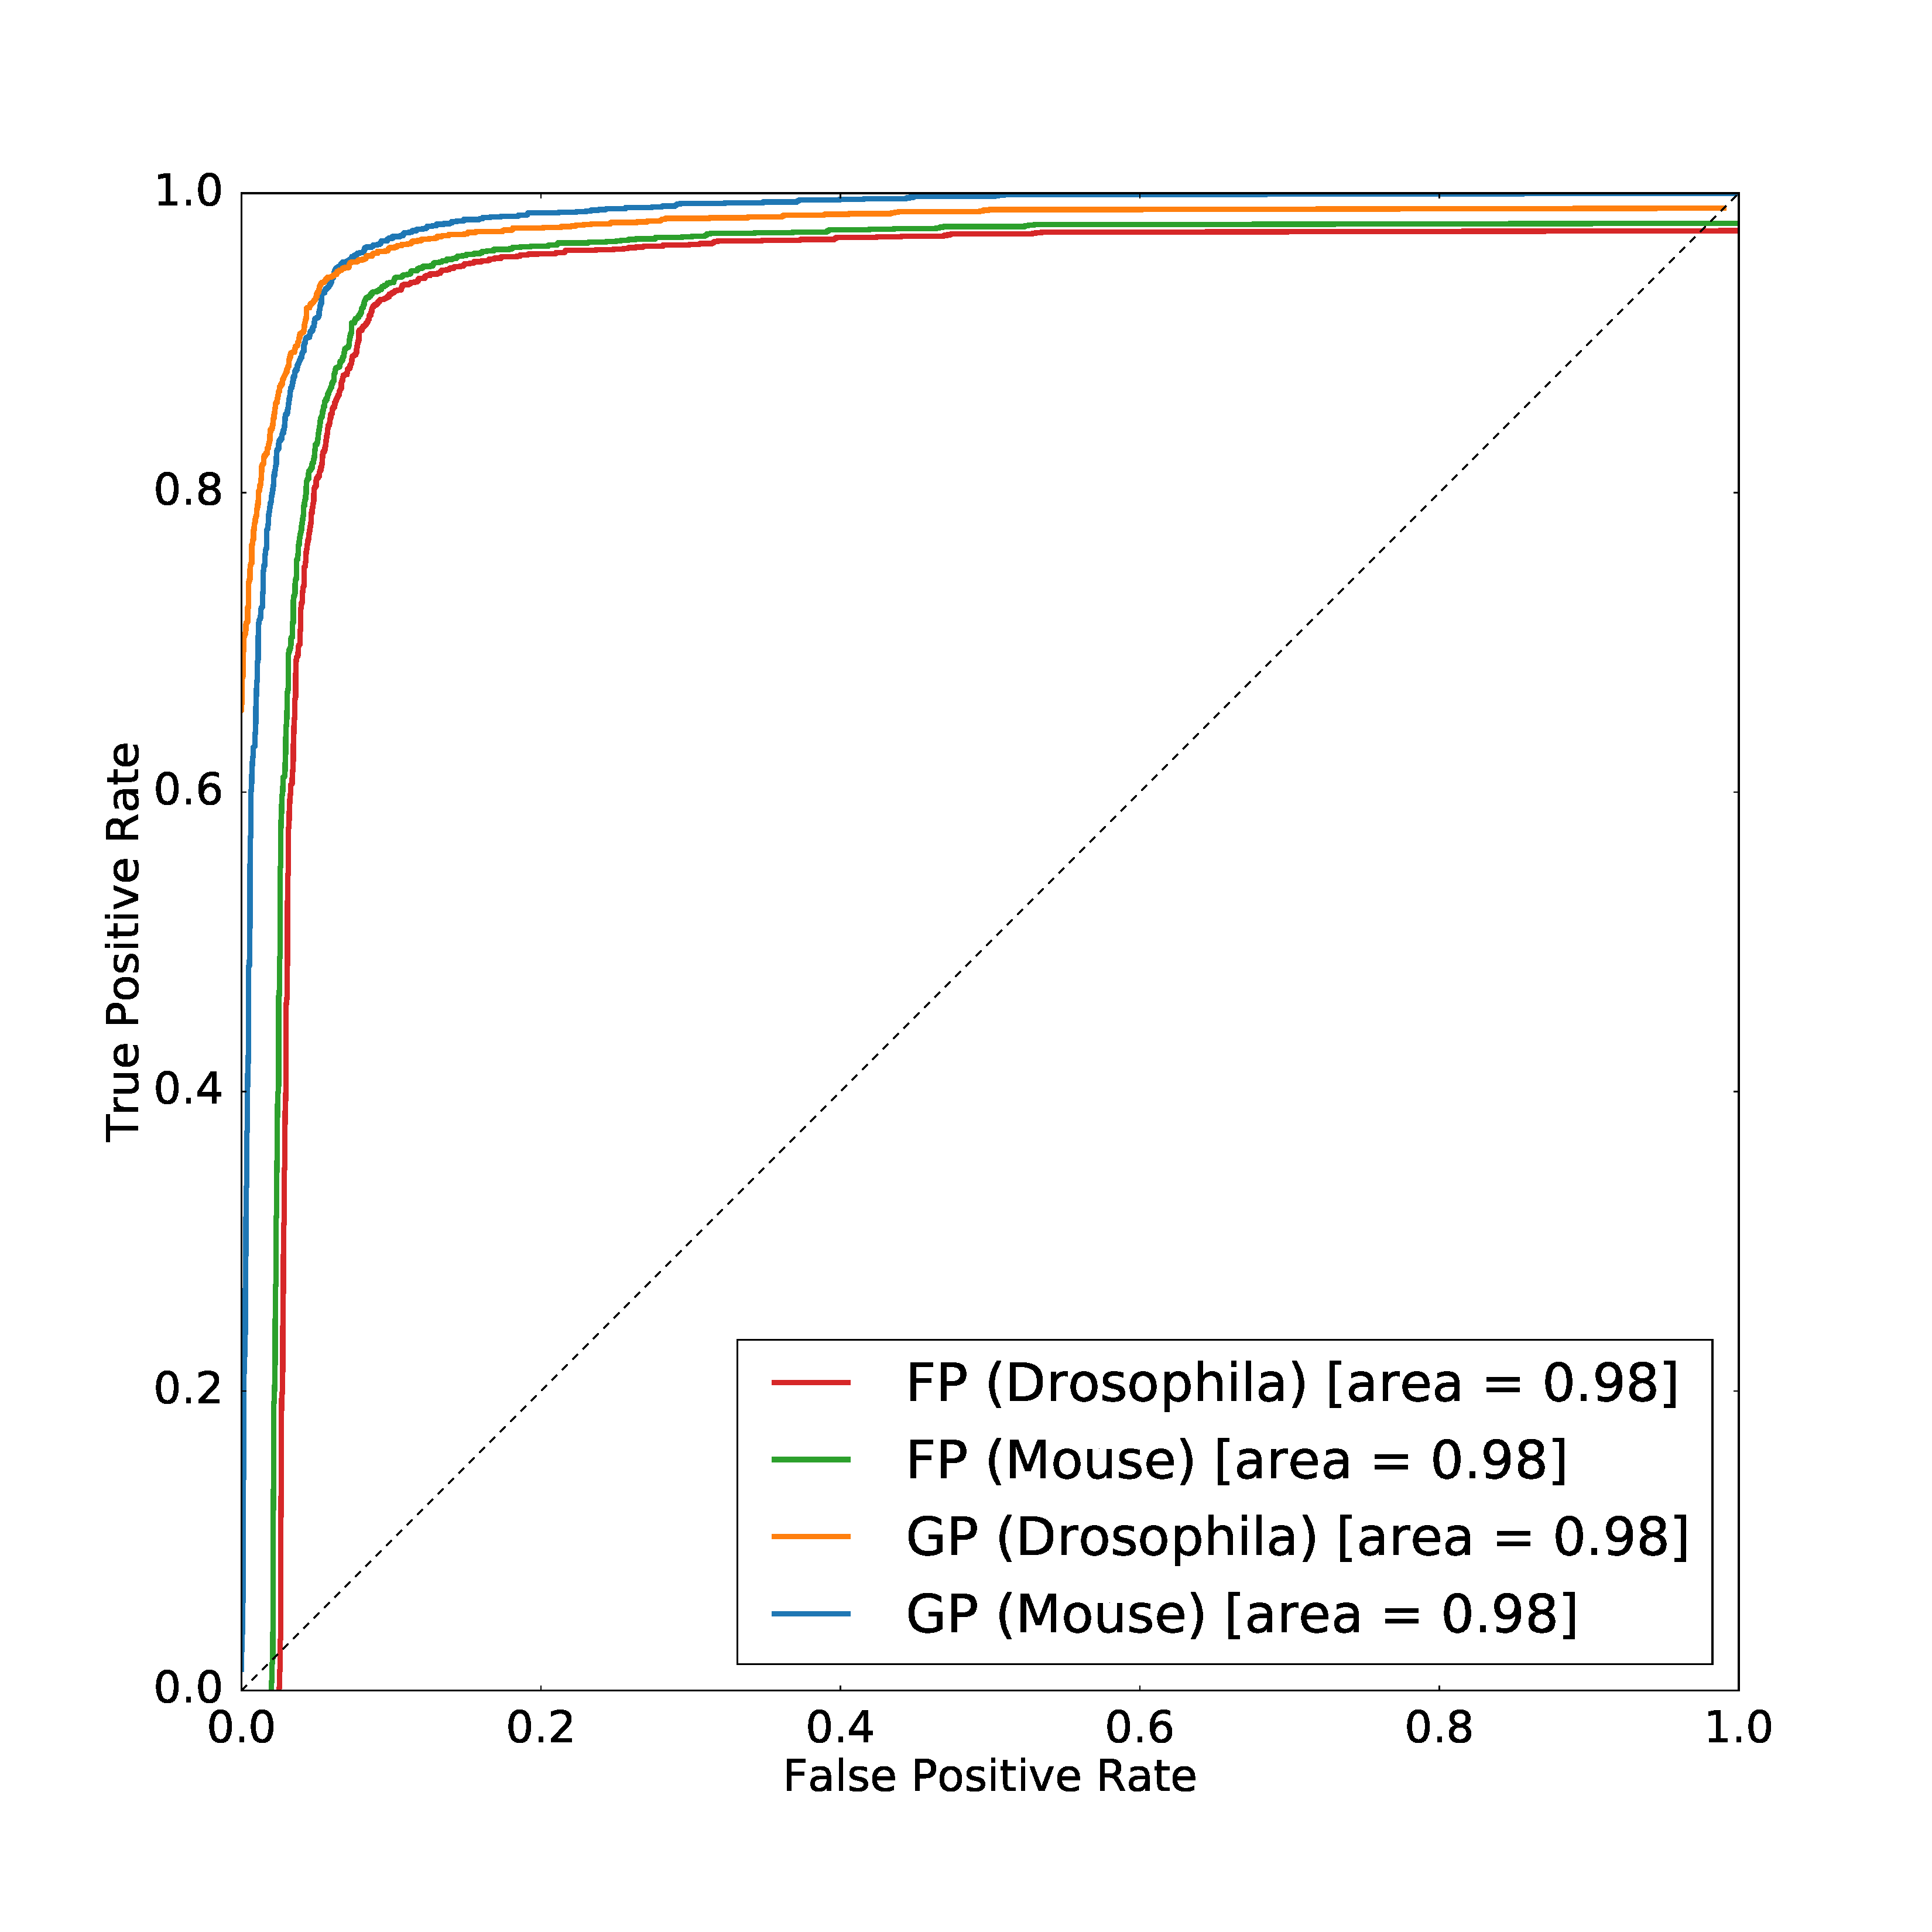
\includegraphics[width=\linewidth]{gfx/roc.pdf}
%\end{center}
%  \vspace{-10mm}
%   \caption{ROC performance of guided proofreading (GP) and focused proofreading (FP) trained separately on mouse and drosophila brain images. The area under the curve indicates better performance for GP.}
%\label{fig:roc}
%\end{figure}

%\subsection{Mouse Brain}
%
%Mouse brain is a common target for connectomics research because the structural proportions are similar to human brains~\cite{jeff_science}. For our first experiment we recruited novice and expert participants as part of a quantitative user study. Our second experiment is performed on a larger dataset and we evaluate a simulated user.
%\\~\\
%\textbf{User study.} Recently, Haehn \etal evaluated the interactive proofreading tools Raveler, Mojo, and Dojo as part of an experiment with novice users~\cite{haehn_dojo_2014}. The participants corrected an automatic segmentation with merge and split errors. The dataset was the most representative sub-volume (based on object size histograms) of a larger connectomics dataset and $400x400x10$ voxels in size. The participants were given a fixed time frame of 30 minutes to perform the correction interactively. While participants clearly struggled with the proofreading task, the best performing tool in their evaluation was Dojo. The dataset including manually labeled ground truth and the results of Haehn \etal are publicly available. This means we are able to use their findings as a baseline for comparison of GP for novices. In particular, we use the best performing user of Dojo who was truly an outlier as reported by Haehn \etal.
%
%Since interactive proofreading most likely yields lower performance than aided proofreading, we also compare against FP by Plaza~\cite{focused_proofreading} which is integrated in Raveler and freely available. For FP we consulted an expert to obtain the best possible parameters as shown in table \ref{tab:parameters}. Besides performance by novices, we are also interested in expert proofreading performance. Therefore, we design between-subjects experiments for 20 novice users and separately, for 6 expert users using the exact same conditions as Haehn \etal. The recruiting, consent and debriefing process is further described in the supplementary material. We randomly assign 10 novices to GP with active label suggestion (GP*) and 10 novices to FP. For the expert experiment, we assign accordingly.
%In addition to human performance, we also evaluate automatic GP, automatic GP with active label suggestion (GP*) and automatic FP. Due to the automatic nature, we do not enforce the 30 minute time limit but we stop once our probability threshold of $p_t=.95$ is reached. This value was observed as stable in previous experiments using automatic GP (see supplementary material). To measure proofreading performance in comparison to ground truth, we use the adapted Rand error (aRE) metric~\cite{RAND}. aRE is a measure of dissimilarity, related to introduced errors, meaning lower scores are better.
%
%The results of our comparisons are shown in the first row of Fig.~\ref{fig:results_mouse}. In all cases, GP* is able to correct the segmentation further than other methods (aRE measures: automatic GP XX, GP* XX, FP XX, novice Dojo XX, GP* XX, FP XX, expert Dojo XX, GP* XX, FP XX). This is not surprising since guided proofreading works for both merge and split errors while FP does not and in interactive Dojo the majority of time is spent finding errors which is minimized for aided proofreading solutions. In fact, the average correction time for novices is for GP* 3.6 (expert X), for FP Y (expert YY), and for Dojo 30 (expert ZZ) seconds.
%\\~\\
%\textbf{Simulated experiment.} For our second experiment with mouse brain data, we proofread the last 50 slices of the blue 3-cylinder mouse cortex volume of Kasthuri \etal~\cite{kasthuri2015saturated} which we also used for testing in section~\ref{sec:methods}. The data was not seen by the network before and includes $2048x2048x50$ voxels with a total number of 17,560 labeled objects. Since an interactive evaluation of such a large dataset would consume a significant amount of time, we restrict our experiment to a simulated (perfect) user and to automatic corrections, both with GP, GP* and FP. Similar to our comparison study, the simulated user assess a stream of errors by comparing the adapted Rand error measure before and after each performed correction. The simulated user is designed to be perfect and only accepts corrections if the measure is reduced. This time, we do not enforce a time limit to see the lower bound of possible corrections. For automatic GP and GP*, we use our defined probability threshold $p_t=.95$.
%
%The results of this experiment are shown in the second row of Fig.~\ref{fig:results_mouse}. GP* is again able to correct the segmentation further than other methods (aRE measures: automatic GP XX, GP* XX, FP XX, simulated GP* XX, FP XX). Again, the results are not surprising since GP* can correct merge and split errors.
%
%\subsection{Drosophila Brain}
%
%The drosophila brain is analyzed by connectomics researchers because of its small size and hence, a reasonable target to obtain a complete wiring diagram. Despite the size, fruit flies exhibit complex behaviors and are in general well studied. We evaluate the performance of our guided proofreading classifiers on three different datasets of adult fly brain. The datasets are publicly available as part of the MICCAI 2016 challenge on circuit reconstruction from electron microscopy images (CREMI)\footnote{The MICCAI CREMI challenge data is available at  http://www.cremi.org}. Each dataset consists of $1250x1250x125$ voxels of training data (A,B,C) as well as testing data (A+,B+,C+) of the same dimensions. Manually labeled ground truth is also available for A,B, and C but not for the testing data.
%
%Since drosophila brain exhibits different cell structures than mouse brain, we retrain the guided proofreading classifiers (and our automatic segmentation pipeline) as well as focused proofreading combined on the three training datasets. We use 300 slices of the A,B,C samples for training and validation, and 75 slices for testing. This results in YYY correct and ZZZ split error patches (respectively, XXX and YYY for testing). The architecture and all parameters of our classifiers stay the same. The trained GP classifier exhibits a reasonable performance on the testing data as seen in Fig.~\ref{fig:roc}.
%
%\begin{figure}[h]
%\begin{center}
%  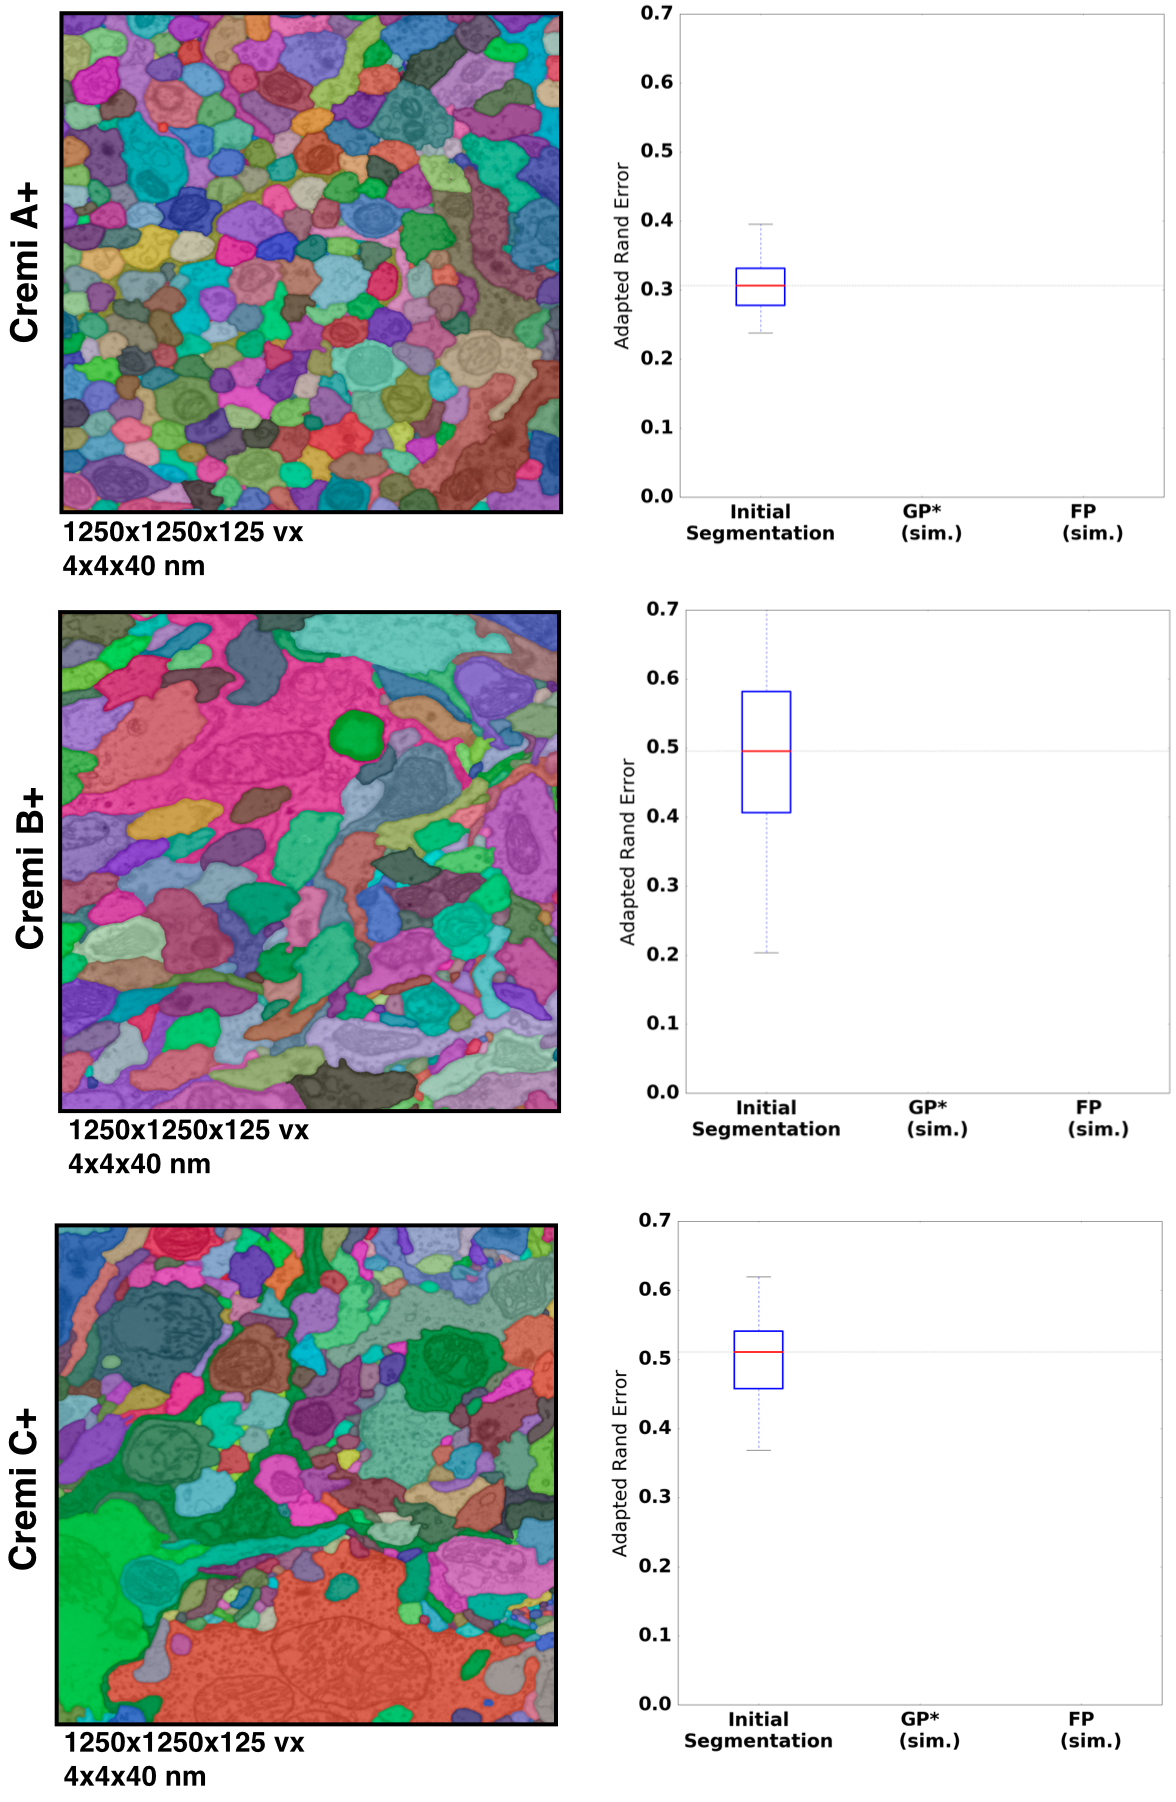
\includegraphics[width=\linewidth]{gfx/results_fruitfly.png}
%\end{center}
%  \vspace{-4mm}
%   \caption{Results of guided proofreading with active label suggestion (GP*) and focused proofreading performed automatically on three drosophila datasets. The datasets are part of the MICCAI 2016 CREMI challenge and publicly available. We measure performance as adapted Rand error (the lower, the better). GP* is able to correct the initial segmentation further than FP. Our GP* scores places us XXnd on the CREMI leaderboard.}
%\label{fig:results_fruitfly}
%\end{figure}
%
%We then use the trained GP* and FP classifiers to evaluate proofreading automatically. Since ground truth labeling is not available, the evaluation is performed by submitting our results to the CREMI leaderboard. Again, we use adapted Rand error to quantify the performance. Fig.~\ref{fig:results_fruitfly} shows the results for each of the A+,B+, and C+ datasets. The performance of GP* is significantly better than FP and places us XXnd on the CREMI leaderboard.


\section{Results and Discussion}

%We measure the performance of proofreading quantitatively by comparing VI scores of segmentations against ground truth labelings. Lower VI scores indicate less distance to the ground truth and a better segmentation. For all experiments, we report the VI score of the initial segmentation followed by the VI score of the proofreading output.
Additional plots and confirmatory data analysis are available as supplemental material due to limited space. 

\subsection{Classification Performance}

\paragraph{L.~Cylinder.} Evaluation was performed on previously unseen sections of the mouse cortex volume from Kasthuri~\etal~\cite{kasthuri2015saturated}. We generated a dataset of 81,184 correct and 8,780 split error patches with respect to the ground truth labeling. Then, we classified each patch by using focused proofreading and guided proofreading, and compare performance (Fig. \ref{fig:pr}). Our method exhibits higher sensitivity and lower fall-out.% for correct and erroneous patches.

%\begin{table}[t]
%\caption{Classifier comparison on an unbalanced test set of the L.~Cylinder volume.}%While the training of our classifier is more expensive, testing accuracy is superior. }
%\resizebox{\linewidth}{!}{
%\begin{tabular}{lrrrr}
%\toprule
% & Precision & Recall & F1 score & Test \# \\ 
%\midrule
%\emph{Focused Proofreading} & ~ & ~ & ~ & ~ \\ 
%~~Correct & 0.93 & 0.31 & 0.47 & 81,184 \\ 
%~~Split error & 0.11 & 0.78 & 0.19 & 8,780 \\ 
%\emph{Guided Proofreading} & ~ & ~ & ~ & ~ \\ 
%~~Correct & 1.00 & 0.93 & 0.96 & 81,184 \\ 
%~~Split error & 0.61 & 0.96 & 0.74 & 8,780 \\ 
%\bottomrule
%\end{tabular} 
%}
%\label{tab:prcyl}
%\end{table}

\begin{figure}[t]
\centering
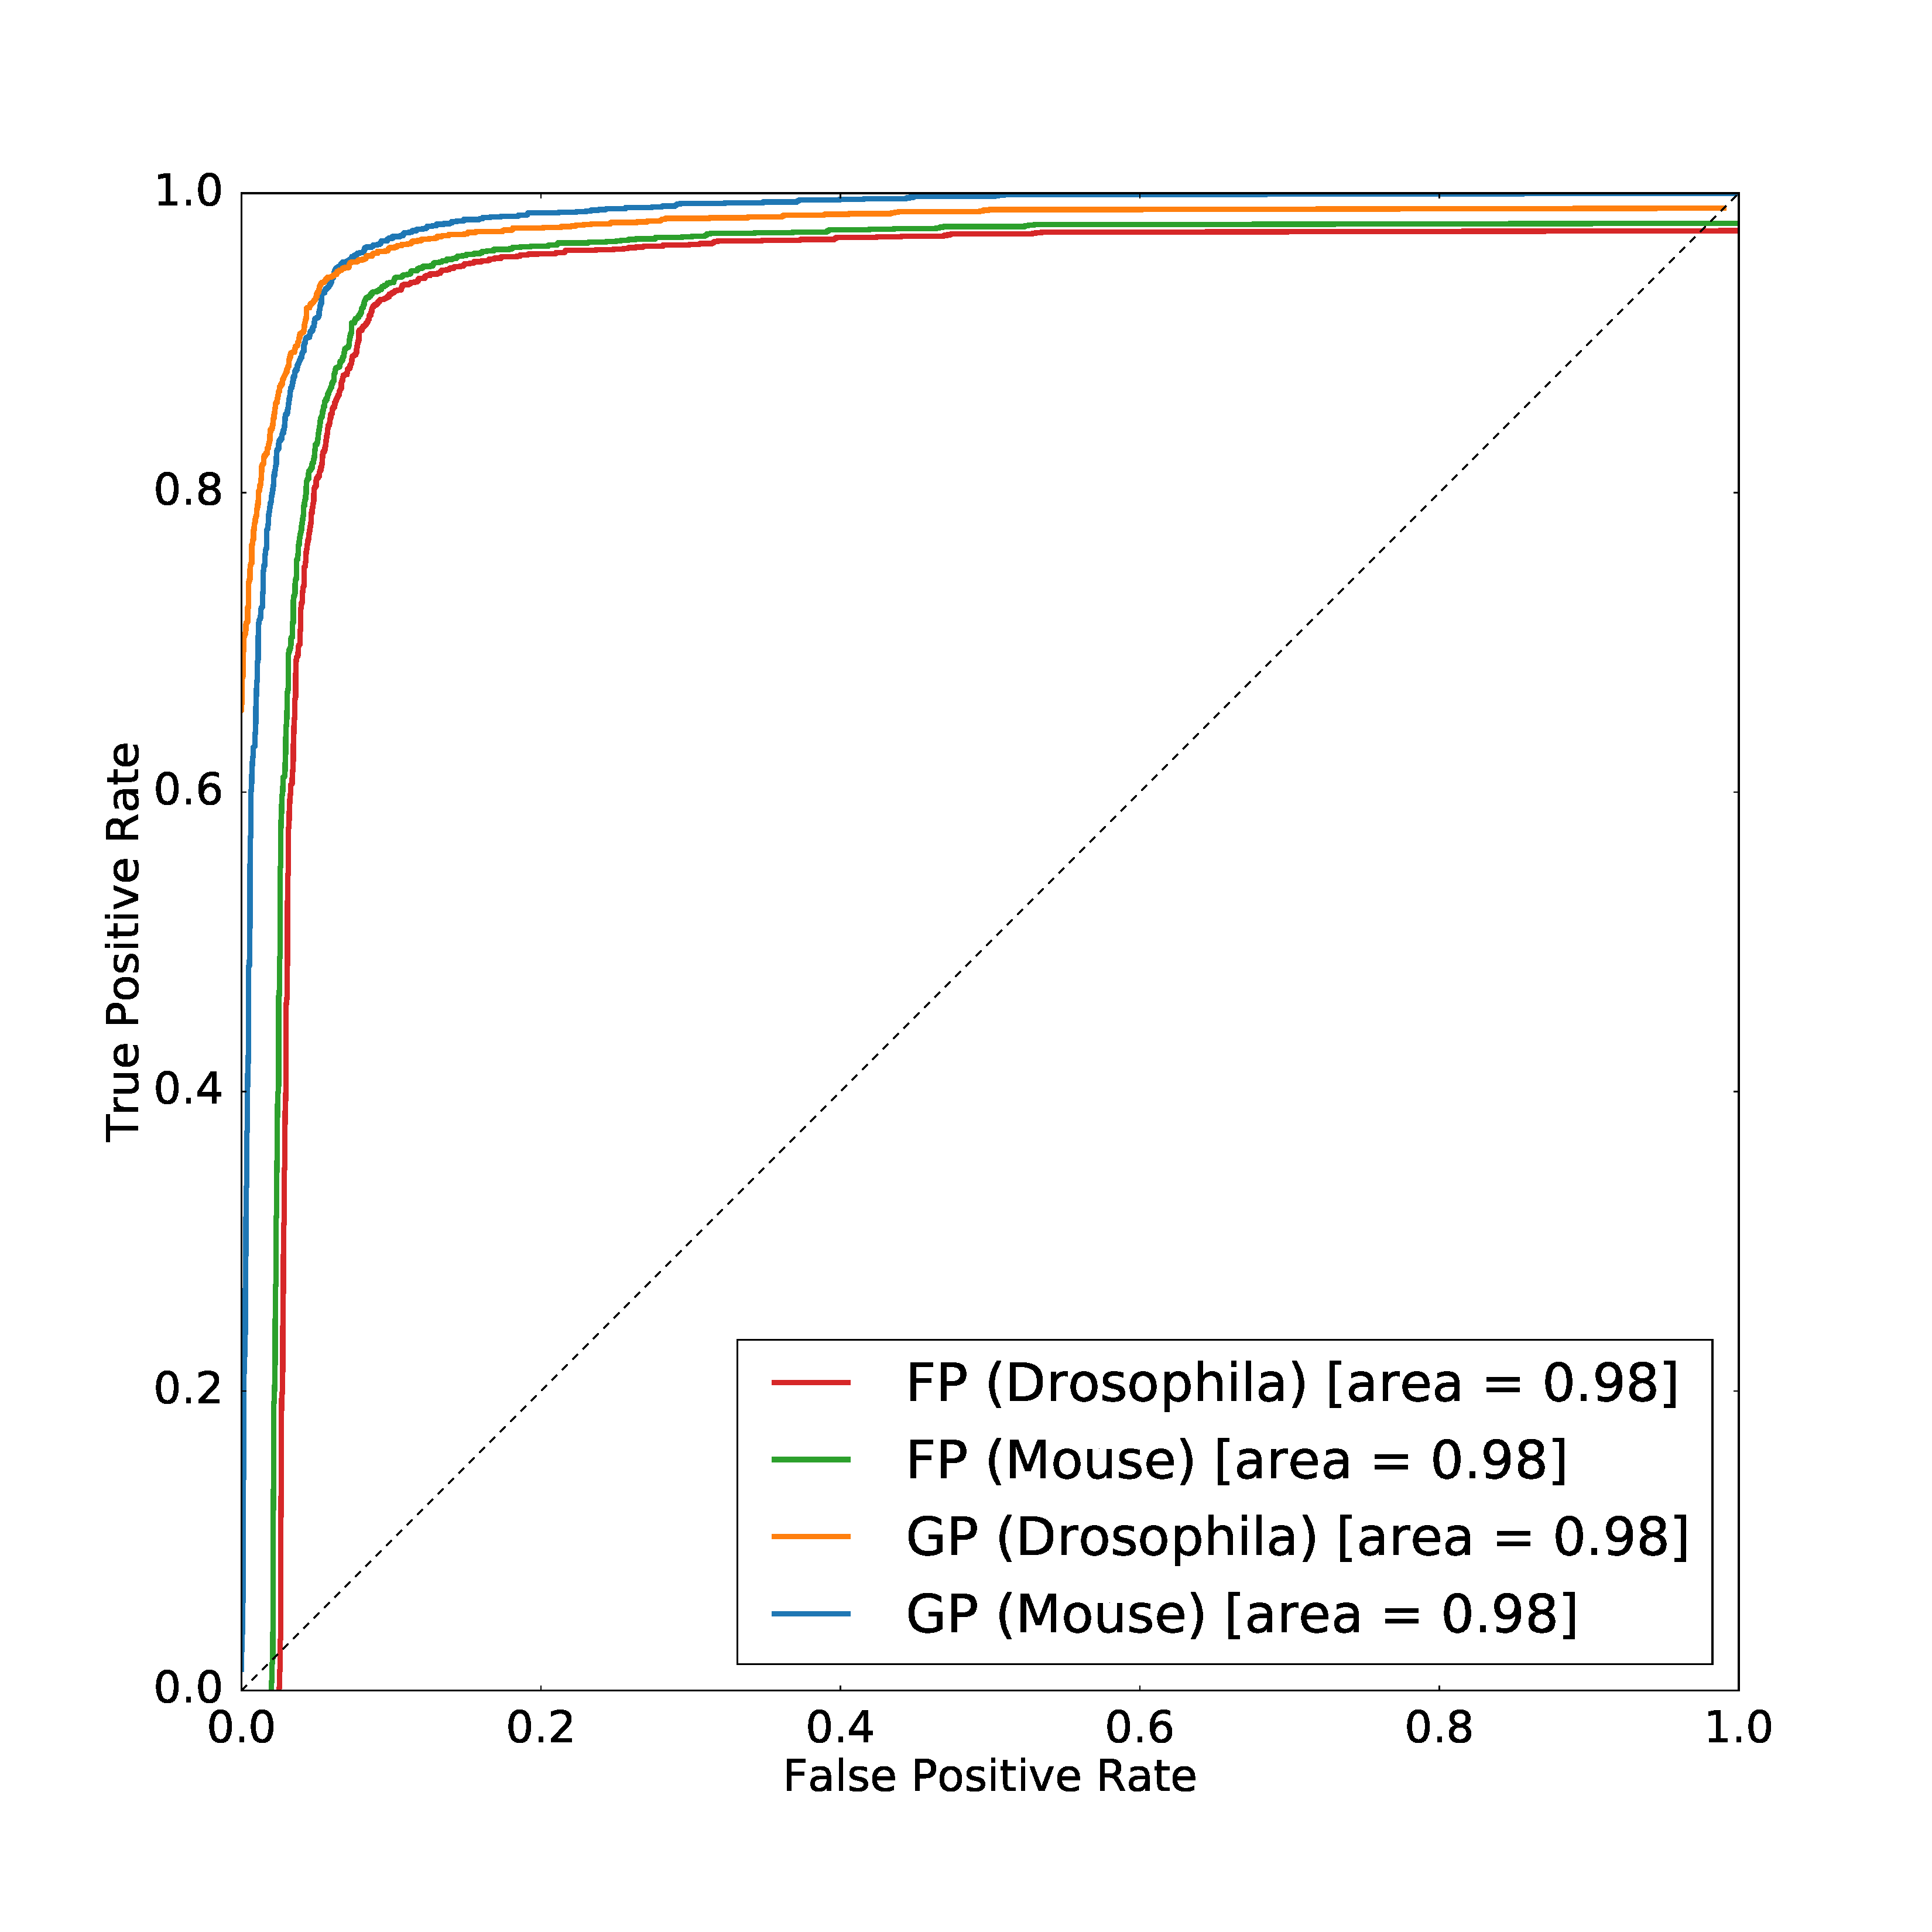
\includegraphics[width=0.9\linewidth]{gfx/roc.pdf}
\caption{Receiver Operating Characteristic curves comparing focused proofreading and guided proofreading automatic correction. We evaluate on unbalanced test sets of the AC4 subvolume (darker colors) and the L. Cylinder volume (lighter colors). Guided proofreading performs better.}
\label{fig:pr}
\end{figure}

\paragraph{AC4 subvolume.} We generated 3,488 correct and 332 error patches (10 merge errors, 322 split errors). Guided proofreading achieves better classification performance (Fig. \ref{fig:pr}).

%\begin{table}[t]
%\caption{Classifier comparison on correct and split error patches of the AC4 subvolume.}%While the training of our classifier is more expensive, testing accuracy is superior. }
%\resizebox{\linewidth}{!}{
%\begin{tabular}{lrrrr}
%\toprule
%& Precision & Recall & F1 score & Test \# \\ 
%\midrule
%\emph{Focused Proofreading} & ~ & ~ & ~ & ~ \\ 
%~~Correct & 0.94 & 0.69 & 0.80 & 3,488 \\ 
%~~Split error & 0.14 & 0.51 & 0.21 & 332 \\ 
%\emph{Guided Proofreading} & ~ & ~ & ~ & ~ \\ 
%~~Correct & 1.00 & 0.92 & 0.96 & 3,488 \\ 
%~~Split error & 0.54 & 0.95 & 0.69 & 332 \\ 
%\bottomrule
%\end{tabular} 
%}
%\label{tab:prac4}
%\end{table}

\subsection{Forced Choice User Experiment}
We performed a user study to evaluate the forced choice error correction method among novices and experts. To be comparable to Haehn~\etal's Dojo user study~\cite{haehn_dojo_2014}, participants were asked to proofread the AC4 subvolume for 30 minutes. We counted 10 merge errors and 322 split errors by computing the maximum overlap of the initial segmentation with respect to the ground truth labeling (provided in \cite{haehn_dojo_2014}). For evaluation, we measure the performance of proofreading quantitatively by comparing VI scores of segmentations. 
%\CHANGED{Our hypothesis is that VI reduction is significantly better with GP than with other tools. For this, we treat VI as a continuous variable and use analysis of variance (ANOVA) followed by parametric tests (Welch's t-test).}
The initial segmentation yields a median VI $=0.476$ ($SD=0.089$), with mean VI $=0.512$ ($SD=0.09$). Most novices and all experts were able to improve upon this score with both focused proofreading and guided proofreading (Fig.~\ref{fig:ac4trails}).

\paragraph{Novice performance.} Participants using focused proofreading were able to reduce the median VI of the automatic segmentation to $0.469$ ($SD=0.87$). On average, users viewed $423.4$ corrections and accepted $45.8$.
%, with an average time of $4.9$ seconds per correction. 
Participants using guided proofreading were able to reduce the median VI to $0.424$ ($SD=0.037$). Here, users viewed on average $353.4$ corrections and accepted $106.9$.
%, with an average correction time of $6.2$ seconds. 
While three users of focused proofreading made the initial segmentation worse, all participants using guided proofreading were able to improve it. In comparison to the results of Haehn~\etal, focused and guided proofreading outperform interactive proofreading with Dojo (median VI $0.535$, $SD=0.055$). The slope of VI score per correction (Fig.~\ref{fig:ac4trails}) and average timings (Tab.~\ref{tab:correctiontimes}) show that guided proofreading enables improvements with fewer corrections than the other tools. Interestingly, novice performance decreases after approximately $300$ corrections. There are two explanations for this: user fatigue, and increasing uncertainty during error suggestion from the classifier. %Regarding fatigue, we suggest that future experiments include short breaks after every ten minutes.

\begin{table}[t]
\caption{Average proofreading speed for novice users of Dojo, Focused Proofreading (FP) and our Guided Proofreading (GP). Our system achieves significantly higher VI reduction per minute (7.5$\times$) over state-of-the-art FP, while being slightly slower per correction.}%While the training of our classifier is more expensive, testing accuracy is superior. }
\resizebox{\linewidth}{!}{
\begin{tabular}{lrrrr}
\toprule
\makecell{Approach\\(Novice)} & \makecell{Time Per\\Correction (s)} & \makecell{VI Reduction\\Per Minute} & \makecell{Improvement} \\
\midrule
\emph{Dojo} & 30.5 & -0.00200 & $-8.7\times$ \\
%\emph{Dojo Expert?} & xxx & xxx \\
\emph{FP} & 4.9 & 0.00023 & $1.0\times$\\
\emph{GP} & 6.2 & 0.00173 & $7.5\times$\\
\bottomrule
\end{tabular} 
}
\label{tab:correctiontimes}
\end{table}

\paragraph{Expert performance.} Domain experts were able to improve the initial segmentation. With focused proofreading, the median VI of the automatic segmentation was $0.439$ ($SD=0.084$). With guided proofreading, the median VI was $0.396$ ($SD=0.032$, Fig.~\ref{fig:ac4boxplot}).


\subsection{Automatic Error Correction}

\paragraph{Selection oracle.} As expected, the selection oracle yields the best performance on all datasets. Fig.~\ref{fig:ac4trails} shows VI reduction using the selection oracle on the AC4 subvolume (initial median VI $0.476$, $SD=0.089$). With focused proofreading, the selection oracle reaches a median VI of $0.353$ ($SD=0.037$) after $1600$ corrections. With guided proofreading, the oracle reaches a minimum median VI of $0.342$ ($SD=0.03$) after $800$ corrections. Both results are close to the best possible median VI of $0.334$ (calculated by computing maximum overlap with the ground truth). The slope of the trails in Fig.~\ref{fig:ac4trails} shows that guided proofreading requires fewer corrections to reach a reasonable reduction in VI. Fig.~\ref{fig:ac4boxplot} shows the VI distribution across methods. On the L.~Cylinder dataset (initial VI $0.379$, $SD=0.118$), focused proofreading reduces the median VI to $0.298$ ($SD=0.075$) after $26,170$ corrections ($2,419$ accepted). Guided proofreading reaches the minimum median VI $0.2996$ ($SD=0.073$) after $10,000$ corrections (in total $27,491$, $2,696$ accepted).

\begin{figure}[t]
\centering
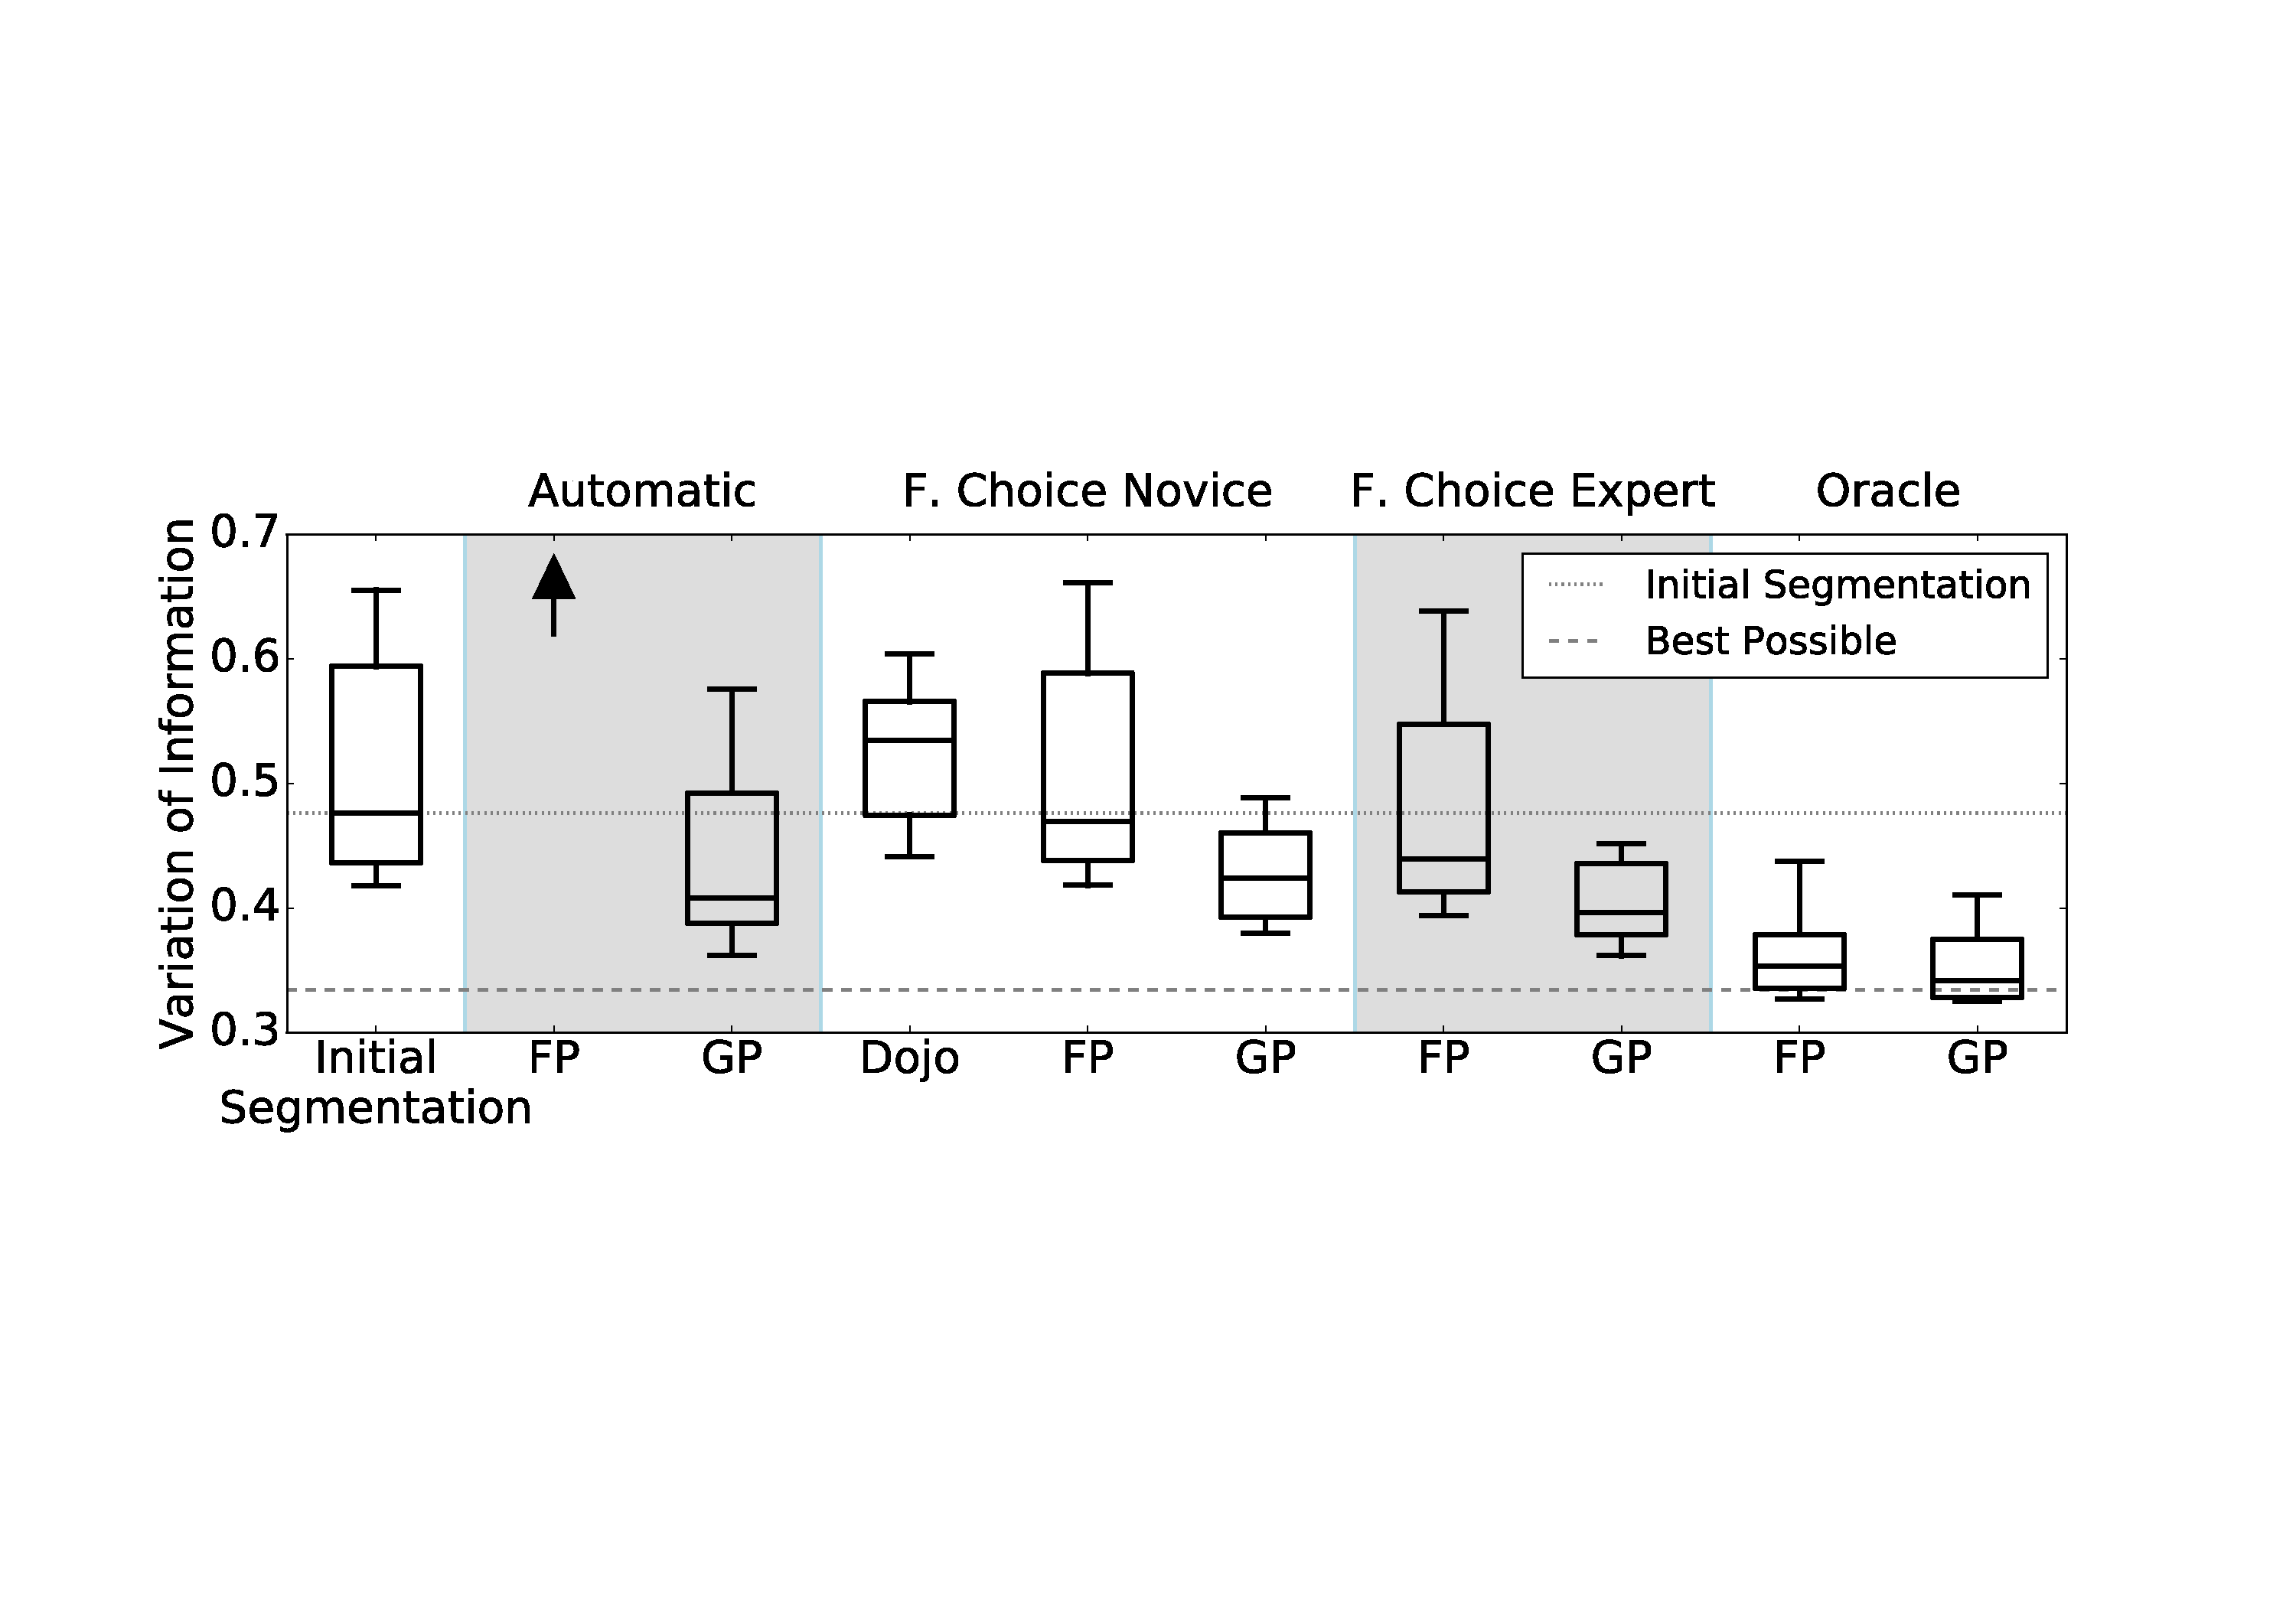
\includegraphics[width=\linewidth]{gfx/ac4boxplot.pdf}
\caption{VI distributions of guided proofreading (GP), focused proofreading (FP) and Dojo output across slices of the AC4 subvolume, with different error correction approaches. The performance of FP with automatic selection is $4.5\times$ higher than GP (\protect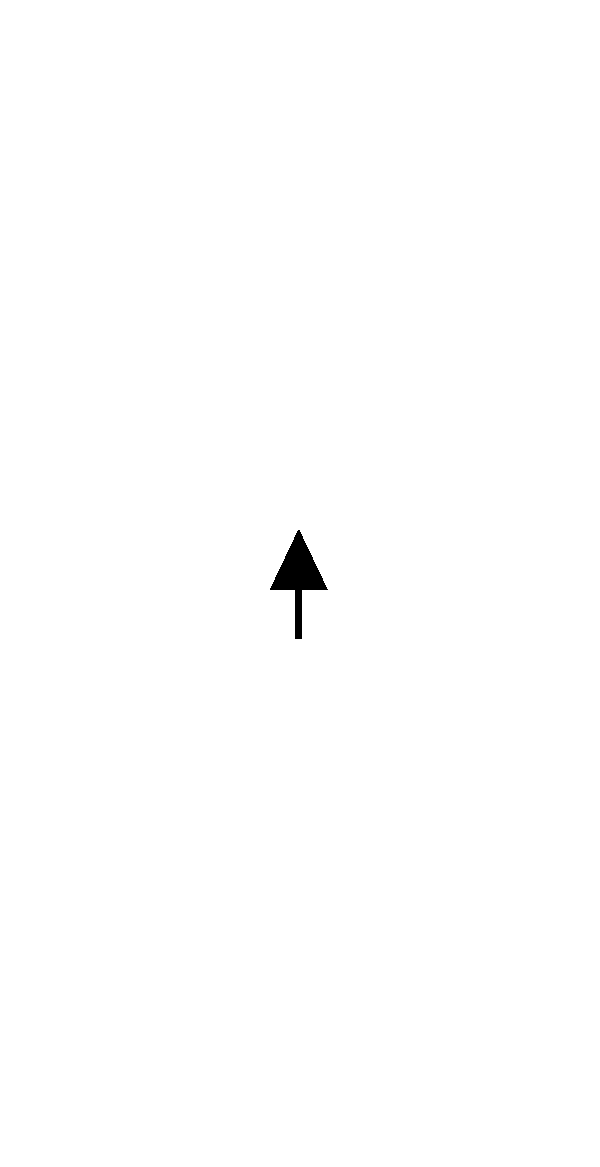
\includegraphics[width=0.2cm]{gfx/arrow.pdf}), with median VI of $1.9$ and $SD=0.496$.}
\label{fig:ac4boxplot}
\end{figure}

\paragraph{Automatic selection with threshold.} Focused proofreading was not designed to run automatically. This explains the poor performance on the AC4 subvolume (VI of $1.9$, $SD=0.496$) and on the L.~Cylinder dataset (VI of $2.75$, $SD=0.789$). For guided proofreading, we set $p_t=0.95$ for both datasets. This reduces median VI in the AC4 subvolume to $0.398$ ($SD=0.068$). This result is comparable to expert performance. Guided proofreading also reduces VI in the L.~Cylinder data to $0.352$ ($SD=0.087$).

\paragraph{Merge Error Detection.} Guided proofreading performs merge error detection prior to split error detection. The classifier found 10 merge errors in the AC4 subvolume, of which 4 reduced VI. Automatic selection with $p_t=0.95$ corrected 6 of these errors (Prec./Recall 0.87/0.80, F1-score 0.80). This was not captured in median VI, but resulted in a mean VI reduction from $0.512$ ($SD=0.09$) to $0.509$ ($SD=0.086$). The selection oracle reduced mean VI with only merge errors to $0.508$ ($SD=0.086$). In the forced choice user study, novices marked 1.9 merge errors for correction and reduced mean VI to $0.502$ (experts marked 2, VI $0.503$, $SD=0.086$). This shows how hard it is to identify merge errors. In 50 sections of the L.~Cylinder dataset, 151 merge errors were automatically found of which 17 reduced VI. Automatic selection with $p_t=0.95$ corrected 6 true VI-reducing errors and 30 VI-increasing ones (Prec./Recall 0.82/0.73, F1-score 0.77) to negligible VI effect. 

\subsection{Proofreading in Connectomics Benchmark}

Along with our classifier code, we also present this evaluation scenario to the community as the first benchmark for proofreading in connectomics. We include representative connectomics data with ground truth labels, all participant results and demographics from the interactive experiments, our complete results from this paper, and standardized metrics for comparing different proofreading approaches. This framework will facilitate further comparisons to help make progress in connectomics (link omitted for review).

%\subsection{Limitations}
%Guided proofreading works on 2D image sections. This enables error correction without a computationally expensive alignment process. However, the output requires an additional (block-)merging step prior to 3D  analysis.


\section{Conclusions}

Humans are the bottleneck when proofreading segmentation data and minimizing the manual labor is the goal. Our classifiers suggest potential errors and corrections better than existing methods. This reduces the time spent finding and correcting errors.
Our experiments also show that automatic proofreading has potential to further reduce human involvement. This will be the target of future research. We provide our framework and data as free and open research at \url{http://rhoana.org/guidedproofreading/}.

\section*{Acknowledgements}
We would like to thank Stephen Plaza for detailed explanations of focused proofreading and Toufiq Parag for the configuration of the NeuroProof classifier.




{\small
\bibliographystyle{ieee}
\bibliography{connectomics}
}

\end{document}
